\chapter{Case Study - Wearable Edge AI towards environmental studies}
\label{chap:ecology}

\nomenclature{VAE}{Variational Autoencoders}
\nomenclature{GAN}{Generative Adversarial Network}
\nomenclature{GRP}{Gaussian Random Process}
\nomenclature{GPE}{Gaussian Process Estimator}
\nomenclature{WLAN}{Wireless Local Area Network}
\nomenclature{MLP}{Multi-Layer Perceptron}
\nomenclature{LIDAR}{Light Detection and Ranging}
\nomenclature{IMU}{Inertial Measurement Unit}

This chapter is dedicated to the evaluation of the case-studies developed towards our first stakeholders. In the introductory section, we defined these target audience as the researchers, students, professors, and practitioners within ecology. We developed applications within three main branches: leaf damage estimation, diseases evaluation and mapping, and ants distribution and couting estimation.

\section{Leaf damage estimation}

The first application in our context is the leaf damage estimation. This information is important for the stakeholders related to the ecological field. For instance, researchers use this variable as an indicator to analyze the ecosystem interactions \cite{muiruri2019forest,benitez2018effect}, or even to analyze the impact of predators in crops \cite{saidov2018first,baudron2019understanding}.

\subsection{Requirements}

The first step in this analysis is evaluating the requirements for the proposed method. For this matter, we display a version of the co-design diagram presented in Figure \ref{fig:simplified-codesign-1}, which is a simplification of the diagram presented in Figure \ref{fig:codesign-2.0}. 

\begin{figure}[ht!]
    \centering
    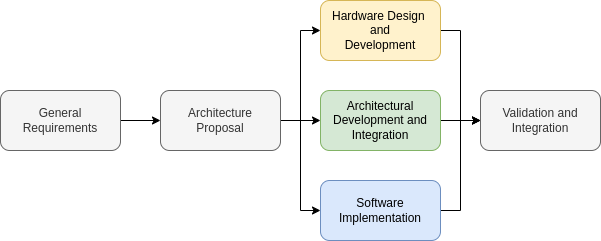
\includegraphics[width = .8\linewidth]{Figures/simplified-codesign.png}
    \caption{Simplified Co-design diagram.}
    \label{fig:simplified-codesign-1}
\end{figure}

This representation displays the need to raise the constraints for the application and classify them into the hardware, software or architectural domain. The constraints identified for this matter are:

\begin{itemize}
    \item The application must reconstruct the leaf shape using artificial intelligence [\textit{Software}].
    \item The application must have a mean to extract a single leaf image from the environment [\textit{Hardware}].
    \item The application must move the captured image into an AI accelerated hardware [\textit{Architecture}].
    \item The image from the leaf must be converted into a mask using image processing [\textit{Software}].
\end{itemize}

Given these constraints, we proposed the usage of a conditional GAN using the Tensorflow environment, allowing the integration with embedded AI accelerated hardware. We also propose the means in which a user can extract a leaf image which can input into such algorithm.

\subsection{Method overview}

\begin{figure}[ht!]
    \centering
    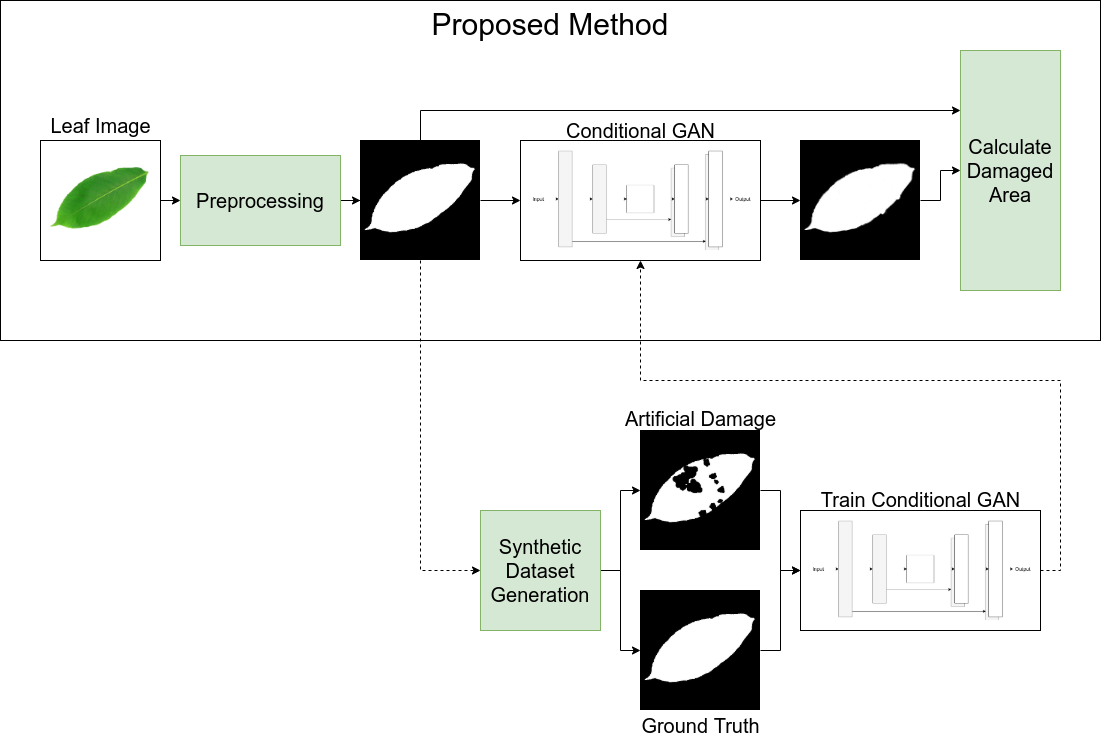
\includegraphics[width = .8\linewidth]{Figures/method-overview.png}
    \caption{Proposed Method and Work Overview}
    \label{fig:method-overview}
\end{figure}

The primary process of our proposed method begins with a preprocessing step that extracts a mask of the leaf area in the image, separating it from the background. The segmented image is then fed into a Conditional GAN model trained to produce an estimated original leaf shape. Lastly, we compare the output with the input image to determine the estimated percentage of defoliation. Figure \ref{fig:method-overview} provides a visual representation of this method.

In addition, we employed the preprocessing method to create a database of masks that includes the complete leaf shapes. These images were utilized to produce a synthetic database that includes leaf masks with artificially induced damage. The latter database was used to train the Conditional GAN method to obtain the test model, utilizing the original masks database as the ground truth. Figure \ref{fig:method-overview} also illustrates this series of stages.

%==========================================
\subsection{Datasets Description}

In this study, we worked with two distinct databases. The first one, referred to as FLAVIA henceforth, was introduced by Wu et al. \cite{wu2007leaf}. This dataset comprises 1907 colored images of leaves from 33 distinct plant species, with a resolution of 1600x1200 pixels. We utilized this dataset to create the synthetic database and for model training, validation, and testing purposes.

The second dataset we used is the Middle European Woods dataset presented by Novotny and Suk \cite{novotny2013leaf}. We will refer to this dataset as MEW 2012 in the rest of the paper. It consists of 9745 images of leaves from 153 different species, already binarized and available in various resolutions. We employed this dataset to conduct additional tests on the shape reconstruction and damage estimation process.

%==========================================
\subsection{Preprocessing}

As previously mentioned, the initial step in the data flow is preprocessing, which aims to extract the image from the background. We employed this technique to create a synthetic database that includes leaf masks with artificially induced damage. Additionally, we utilized the preprocessing method to generate a database of masks that includes the complete leaf shapes. The preprocessing stage comprises six consecutive steps:

\begin{enumerate}
    \item Convert to grayscale;
    \item Insert paddings to turn the image into a square shape;
    \item Reduce the size of the image to 400x400;
    \item Enhance the contrast using a radiometric transformation;
    \item Calculate the threshold using Otsu's method;
    \item Binarize the image;
\end{enumerate}

The initial step involves converting the image colorspace to grayscale. We then add padding to the image to shape it into a square. The padding is selected based on the highest pixel value to improve binarization performance when using thresholding algorithms. Following this, we employ a radiometric transformation to enhance the image contrast, as per Equation \ref{eq:radtransf}. In this equation, $G_i(x,y) \in [0,1],$ and $G_i(x,y) \in \mathbb{R}$ represent the normalized pixel values of the original image. It is worth noting that $G_f(x,y) \in [0,1],$ and $G_f(x,y) \in \mathbb{R}$ represent the output process parameters.

\begin{equation}
\label{eq:radtransf}
    G_f(x,y) = G_i(x,y)^{10}.
\end{equation}

Following the contrast enhancement stage, we move on to binarization. To achieve this, we utilized Otsu's method \cite{otsu1979threshold} to identify the separation threshold between the leaf and the background. This method works by minimizing the intra-class variance function, as defined in Equation \ref{eq:intraclass-variance}.

\begin{equation}
\label{eq:intraclass-variance}
    \sigma^2_b(k) = \frac{[\mu_T\omega(k)-\mu(k)]^{2}}{\omega(k)(1-\omega(k))}
\end{equation}

Where $k$ is the highest number of all the possible threshold values and:

\begin{align}
    \omega(k) = \sum_{i = 1}^{k}p(i);\\
    \mu(k) = \sum_{i = 1}^{k}i \dot p(i);\\
    \mu_T = \sum_{i = 1}^{L}i \dot p(i).
\end{align}

The values required for this method are obtained from the histogram, normalized as a probability density function represented by $p(i)$, for the $L$ candidate threshold values in the histogram. This approach provides a reliable estimation for the threshold value required to segment the image from its background. In this equation, $\omega(k)$ represents the class probability, $\mu(k)$ represents the class means, and $\mu_T$ represents the global mean. The variable $i$ represents all possible pixel values present in the histogram. Assuming every possible value of $k$ falls within the range of $[0,255]$ and is a natural number, all possible values of $i$ should be $i \in [1,255],$ $i \in \mathbb{N}$.

We also used this method to prepare the synthetic database, which was employed to train the conditional GAN method to obtain the test model using the original masks database as the ground truth. During the synthetic dataset generation, we removed internal holes to create ideal leaf images. Additionally, we developed a novel method for creating randomly artificial damaged leaf images, which we used to generate a dataset for training the conditional GAN.

%==========================================
\subsection{Synthetic Dataset Generation}

As previously mentioned, the preprocessing pipeline was utilized in the synthetic dataset generation process. We employed this method to prepare the images from the dataset for the application. In this section, we present the pipeline involved in producing images with synthetic damage and the processes included in this pipeline.

Most leaves in the dataset are undamaged, while some may show slight damage or light reflection spots. To better represent the ideal leaf shape, we selected the largest contour recognized after binarization to create a complete leaf representation. Using this technique, we generated 1907 masks corresponding to the 1907 images in the dataset. To create a supervised learning dataset in the next stage, we needed to introduce artificial measurable damage into the leaf masks.

In this stage, we discuss how we created artificial random damage on the leaves. Similar to Da Silva et al. \cite{da2019estimating}, we applied artificial damage techniques to generate a training dataset. We initially assumed that the leaf had a slightly higher probability of having damage at its borders. Therefore, we created a 2-D probability distribution, $g(x,y)$, centered on the $(x_0,y_0)$ average center position of the $x$ and $y$ coordinates of the binarized leaf mask image. Equation \ref{eq:gauss} represents this 2-dimensional Gaussian distribution centered at $(x_0,y_0)$, with a standard deviation of $\sigma$.

\begin{equation}
\label{eq:gauss}
    g(x,y) = e^{-\frac{(x-x_0)^2 + (y-y_0)^2}{2 \dot \sigma^2}}.
\end{equation}

Furthermore, we created a probability function $p(x,y)$, for the damage using $g(x,y)$ according to the following equation:

\begin{equation}
    {p}(x,y) = \frac{1-g(x,y)}{2} + P_0.
\end{equation}

In this scenario, $P_0$ represents the minimum probability offset. The probability of damage beyond the leaf's boundaries in the image must be zero. This condition is achieved by multiplying the probability function by the leaf mask. During the first stage of this study, we selected a baseline value of $P_0 = 0.3$ and $\sigma = 100$, based on practical tests conducted on the databases. In the second stage, we opted for a baseline value of $P_0 = 0.6$ and $\sigma = 10000$, to generate more damage on average. Figure \ref{fig:leaf_pdf} illustrates the probability function for one of the leaves in our dataset.

\begin{figure}[h!]
    \centering
    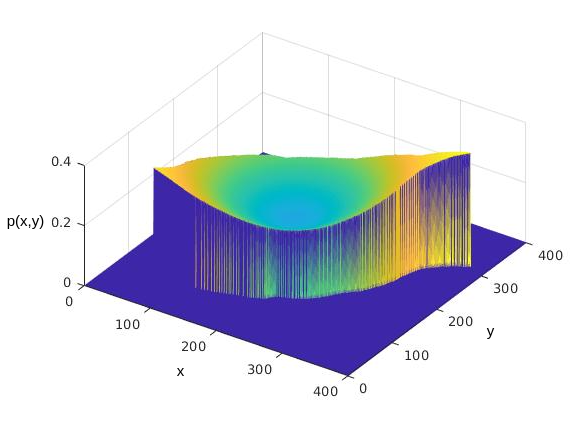
\includegraphics[width = .55\linewidth]{Figures/leaf_pdf.png}
    \caption{Example of damage probability density distribution. This function is used to generate the artificial damage.}
    \label{fig:leaf_pdf}
\end{figure}

\begin{figure}[h!]
    \centering
    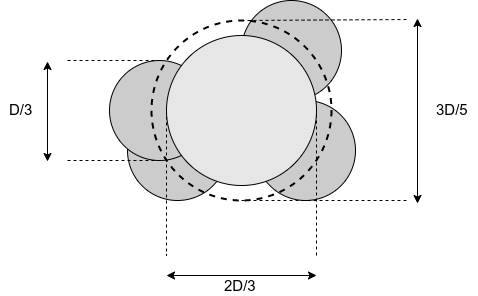
\includegraphics[width = .45\linewidth]{Figures/artificial-damage.png}
    \caption{Illustration of the punctual artificial damage generation method \cite{iceis21leaf}.}
    \label{fig:artificial-damage}
\end{figure}

The damage generated at a point follows a certain rule. Initially, we draw a circle with a diameter of $2D/3$ for a given reference size of $D$. Subsequently, we draw four circles with a diameter of $D/3$, centered at random points located over a virtual circle with a diameter of $3D/5$. Figure \ref{fig:artificial-damage} depicts the punctual artificial generation method.

The artificial damage generation algorithm selects several random coordinates and checks the function to determine whether it should insert damage at that point. If the answer is positive, it injects the loss at the spot by randomly selecting a reference size.

To create the synthetic dataset, we generated 12 versions of each leaf with random losses. We selected a pixel located at a coordinate $(x,y)$ as a candidate for receiving the artificial damage. Damage occurs only if the pixel is located within the leaf boundaries. For the first four images, we ran the method with 100 coordinates. For the fifth to eighth images, we executed the procedure with 200 coordinates. For the final four images, we performed the process with 300 coordinates. The resulting dataset consisted of 22884 shapes with varying levels of artificially generated damage.

%==========================================
\subsection{Conditional GAN Architecture}

Our implementation takes the work of Isola et al. \cite{isola2017image} as a baseline. For this matter, we applied a U-Net-based conditional GAN architecture. This network has two main modules: a generator and a discriminator. At first, the generator takes an input image and produces a predicted output. Then, the discriminator evaluates the prediction.

In this work, the main architecture is based on a U-Net. U-Nets are generative models of deep neural networks. Originally, this technique was proposed to perform segmentation in biomedical images \cite{ronneberger2015u}. They are similar to Variational Autoencoders (VAEs) \cite{hou2017deep}, and due to their generative capability, they can be used to reconstruct images pixel-by-pixel. These networks are applied for recognition and segmentation \cite{dong2017automatic,oktay2018attention} and for reconstruction \cite{hyun2018deep,antholzer2018photoacoustic}.

\subsubsection{Generator}

The generator's architecture is based on an Encoder-Decoder network. For this implementation, a U-Net was used, which has interconnected mirrored layers. The encoder consists of 8 layers (256x256, 128x128, 64x64, 32x32, 16x16, 8x8, 4x4, 2x2), with batch normalization in the intermediate layers. The output also has 8 layers (1x1, 2x2, 4x4, 8x8, 16x16, 32x32, 64x64, 128x128), with batch normalization in the intermediate layers.


\subsubsection{Discriminator}

On the other hand, the discriminator follows a PatchGAN architecture, which is similar to the encoding section of an encoder-decoder network. In this implementation, the discriminator consists of 5 layers (256x256, 128x128, 64x64, 32x32, 31x31), with batch normalization between the intermediate layers. 

\subsubsection{Training}

The network uses a two-part training method. Initially, the discriminator is trained based on the baseline answers. After that, the generator weights are updated based on the baseline truth and the discriminator guess. The training algorithm was performed for 20 epochs, with the first results being better than the ones presented in the literature. However, to avoid overfitting, the network was trained for an additional 5 epochs, which resulted in a significant improvement. As a result, the error becomes much smaller, making it state-of-the-art on the proposed problem.

%=========================================
\subsection{Damage Estimation}

In the previous section, we discussed the network architecture and its training process. In the preprocessing stage, the image is first converted to grayscale and then subjected to a binarization process. The resulting image is then used as input for the conditional GAN, which produces a mask that represents the predicted original shape. Finally, to calculate the damage percentage, we use the following formula:

\begin{equation}
	P_d = (1 - \frac{\sum_{i,j} Im_d(i,j)}{\sum_{i,j} Im(i,j)}) \times 100 (\%).
\end{equation}

Here, $P_d$ represents the damage percentage, $\sum_{i,j} Im_d(i,j)$ represents the sum of the binarized value (0 or 1) of each pixel of the damaged leaf image, and $\sum_{i,j} Im(i,j)$ represents the sum of the binarized value (0 or 1) of each pixel of the baseline image. We used the original image mask as the baseline for calculating the ground truth values of damage, while the model's outputs were used to calculate the predicted damage.

%==========================================
\subsection{Evaluation Methods}

In the previous section, we discussed the neural network used to estimate the original shape of damaged leaves, as well as the image datasets and artificial damage generation process used to create the synthetic dataset. In this section, we will focus on the methods used to evaluate the prediction quality.

We started with 22884 original images and used the first 22833 for our analysis. These images were randomly divided into three separate sets: 10\% for validation, 10\% for testing, and the remaining 80\% for training the algorithm. In the second stage, we repeated the process with modified parameters that allowed for more damage. We also used the 22884 images to create a dataset with the same proportions.

After training the model, we performed a round of predictions on the MEW 2012 dataset. To speed up the generation process, we reduced the images to 256x256 pixels and randomly applied 10 to 40 damage coordinates with a probability of $P_0 = 0.7$, resulting in a total of 38980 images. Although the generation process differed slightly, the images had to be resized to 400x400 pixels to be used with the model.

\subsubsection{Damage Estimation Evaluation}

Similar to Da Silva et al. \cite{da2019estimating}, we calculated the real defoliation percentage $d_r$ and the estimated defoliation percentage $d_e$. These values were measured on both the validation and test sets, as we generated the synthetic dataset from the ground truth. We evaluated the Root Mean Square Error (RMSE), which is calculated using the following equation:

\begin{equation}
	\label{eq:RMSE}
	RMSE = \sqrt{\frac{1}{n} \sum (d_e - d_r)^2}.
\end{equation}

Furthermore, we conducted a series of quantitative and qualitative analyses based on the prediction results.

\subsubsection{Shape Reconstruction Evaluation}

In the previous subsection, we discussed the evaluation method used for the damage estimation process. In addition to analyzing the quality of the defoliation estimation method, we also conducted a quantified evaluation of the image reconstruction process. To do this, we employed the dice coefficient, which is a widely used method for evaluating image similarity \cite{gencctav2012unsupervised,sampat2009complex,shamir2019continuous,mun2017comparison,nitsch2019automatic}. This measurement is used to compare areas and can be easily applied using binarized images. The dice coefficient ($DC$) is calculated for a pair of images ($A$ and $B$) using the following equation:

\begin{equation}
	\label{eq:dice}
	DC = \frac{2 \|(A \cap B)\|}{\|A\| +\|B\|}
\end{equation}

The resulting coefficient value is always in the range of [0, 1]. A high dice coefficient value indicates that the images are highly similar. Therefore, we used this factor to measure the success of the shape reconstruction process by calculating the dice coefficient to compare the ground truth and model output images.

%==========================================
\subsection{A Broader Evaluation on the Damage Estimation Results}

In the previous section, we discussed the method used to evaluate the leaf damage predictions, which involves estimating the original leaf shape using a Conditional GAN. In this section, we provide a broader overview of the original and predicted data to demonstrate the robustness of the proposed solution.

The first important set of results came from analyzing the RMSE values, which were defined by equation \ref{eq:RMSE}. The validation dataset had an RMSE value of 0.92 ($\pm$ 1.90), while the test dataset had a value of 0.92 ($\pm$ 1.85). As we previously mentioned, both the validation and test datasets had similar results for the RMSE value. After the second training stage, the error values were even lower. The validation dataset had an RMSE value of 0.61 ($\pm$ 0.99), and the test dataset had a value of 0.52 ($\pm$ 0.73). As previously shown, these results alone represent a significant improvement over the state-of-the-art. Table \ref{tab:RMSE} presents the results obtained.

\begin{table}[h!]
\caption{\label{tab:RMSE} RMSE Results}
\centering
\begin{tabular}{|l|l|l}
%\cline{2-3}
\hline
 & \multicolumn{1}{|c|}{Validation Set} & \multicolumn{1}{c|}{Test Set} \\ \hline
\multicolumn{1}{|c|}{Initial Round} & 0.92 ($\pm$ 1.90) \%& \multicolumn{1}{c|}{0.92 ($\pm$ 1.85) \%}\\ \hline
\multicolumn{1}{|c|}{Improved Round} & 0.61 ($\pm$ 0.99) \%& \multicolumn{1}{c|}{0.52 ($\pm$ 0.73) \%}\\ \hline
\end{tabular}
\end{table}


\begin{figure}[h!]
    \centering
    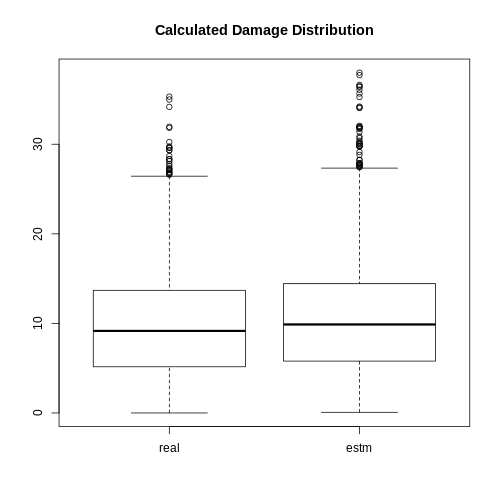
\includegraphics[width = .45\linewidth]{Figures/v1-val-dmgdst.png}
    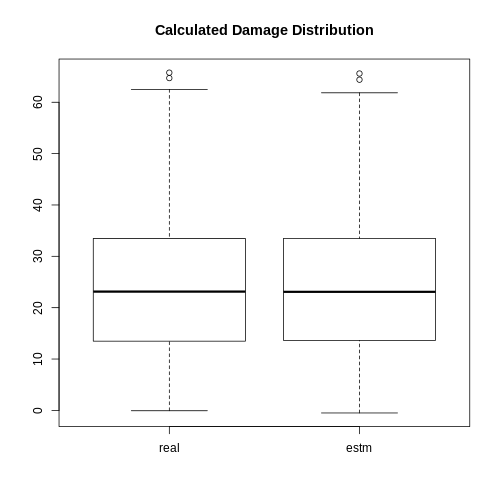
\includegraphics[width = .45\linewidth]{Figures/v2-val-dmgdst.png}
    \caption{Validation Set - Damage Distribution for the Initial and Improved Rounds. }
    \label{fig:validation_dist}
\end{figure}

For the initial stage, the validation set comprised 2283 randomly selected images from the original dataset. The estimated average damage on this set was 10.68 $\pm$ 6.34\%, with a maximum damage value of 37.99\%. The real average damage was 9.86 $\pm$ 6.03\%, with a maximum value of 35.31\%. In the second stage, the validation set contained 2288 randomly selected images from the original dataset. The estimated average damage on this set was 23.88 $\pm$ 12.97\%, with a maximum damage value of 65.59\%. The real average damage was 23.84 $\pm$ 13.06\%, with a maximum value of 65.76\%. The distribution plots for this data are shown in Figure \ref{fig:validation_dist}.

Additionally, we created a graph comparing the obtained data with the ground truth for both the initial and improved stages. Figure \ref{fig:validation_results} displays the results for the validation dataset in both rounds.

\begin{figure}[h!]
    \centering
    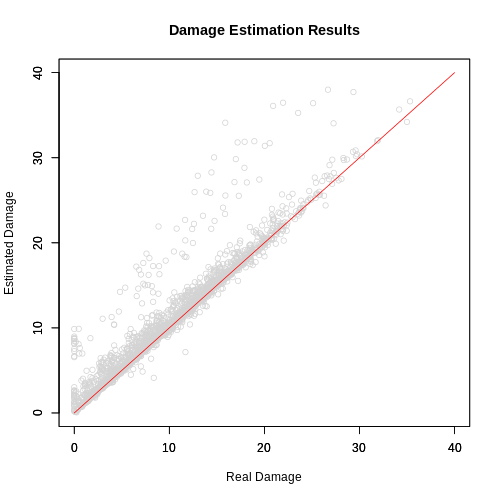
\includegraphics[width = .45\linewidth]{Figures/v1-val-estm.png}
    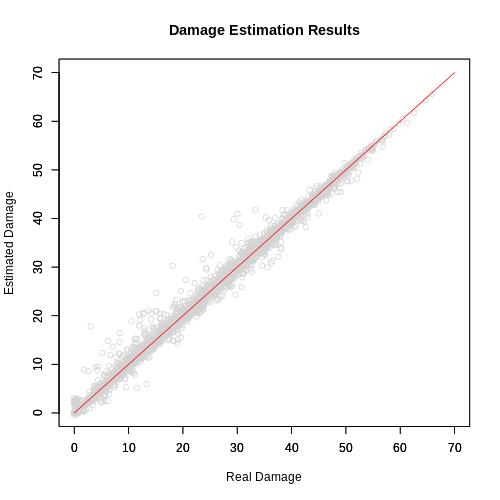
\includegraphics[width = .45\linewidth]{Figures/v2-val-estm.png}
    \caption{Validation damage estimation results for the Initial and Improved Rounds}
    \label{fig:validation_results}
\end{figure}

\begin{figure}[h!]
    \centering
    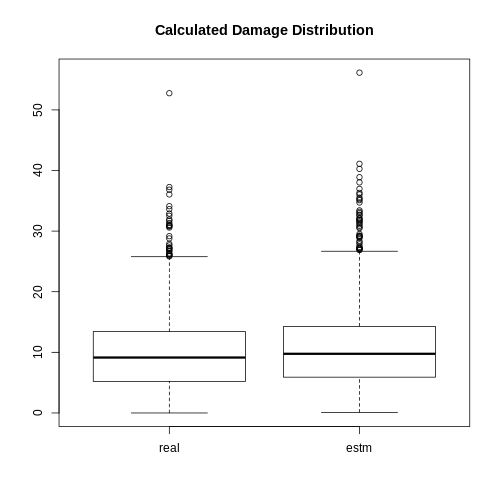
\includegraphics[width = .45\linewidth]{Figures/v1-tst-dmgdst.png}
    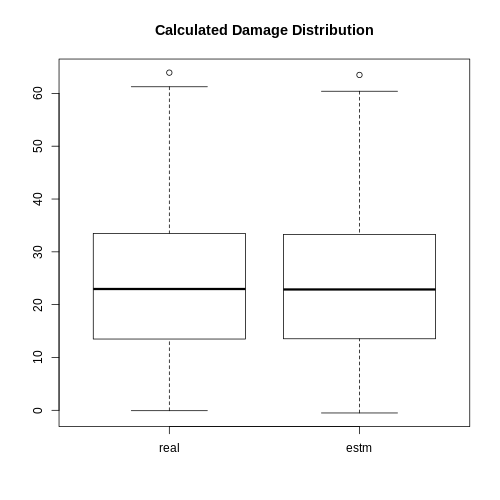
\includegraphics[width = .45\linewidth]{Figures/v2-tst-dmgdst.png}
    \caption{Test Set - Damage Distribution for the Initial Round}
    \label{fig:test_dist}
\end{figure}

Similarly, the test set comprised 2283 randomly selected images from the initial set. The average estimated damage in this set was 10.66 $\pm$ 6.44\%, with a maximum value of 56.14\%. The real damage distribution average and standard deviation were 9.84 $\pm$ 6.19\%, with a maximum damage of 52.74\%. In the second stage, the test set contained 2289 images. The average estimated damage in this set was 23.61 $\pm$ 12.99\%, with a maximum value of 63.49\%. The real damage distribution average and standard deviation were 23.68 $\pm$ 12.99\%, with a maximum damage of 63.92\%. The boxplots with the distribution of this data are shown in Figure \ref{fig:test_dist}.


\begin{figure}[h!]
    \centering
    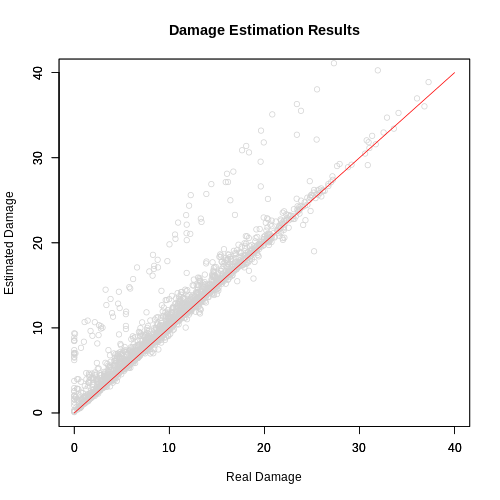
\includegraphics[width = .45\linewidth]{Figures/v1-tst-estm.png}
    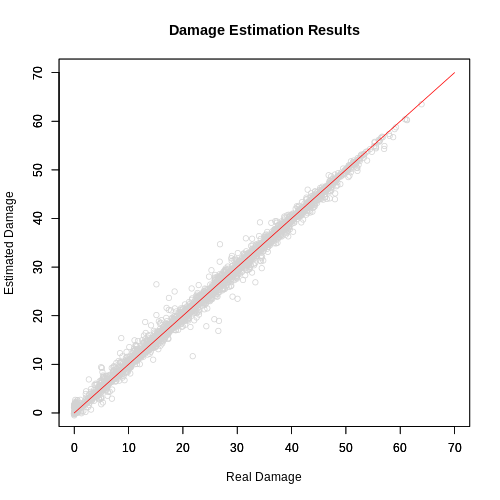
\includegraphics[width = .45\linewidth]{Figures/v2-tst-estm.png}
    \caption{Test set damage estimation results for the Initial Round}
    \label{fig:test_results}
\end{figure}

We also created a graph comparing the obtained data with the ground truth for the test dataset in both the initial and improved stages. Figure \ref{fig:test_results} displays the results. A qualitative analysis of the results indicates that the distributions of the sets are similar, which reinforces the RMSE parameter results.

\subsubsection{MEW 2012 Results}

As previously mentioned, we also conducted predictions on another database containing different species from the ones used during training. We selected MEW 2012, which comprised 9745 images, and generated 38980 images with artificial random damage for this purpose. 

\begin{figure}[h!]
    \centering
    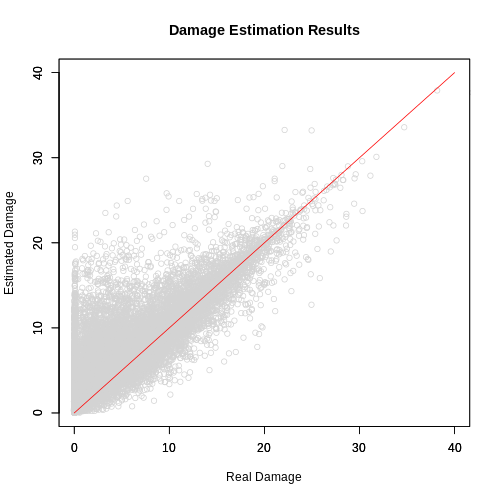
\includegraphics[width = .45\linewidth]{Figures/v1-mew2012-estm.png}
    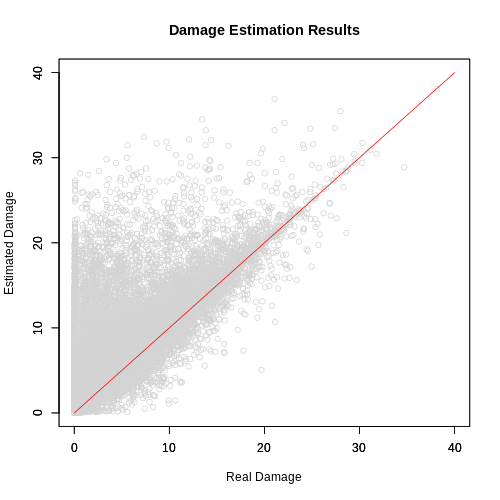
\includegraphics[width = .45\linewidth]{Figures/v2-mew2012-estm.png}
    \caption{MEW 2012 set damage estimation results for the Initial and Improved rounds}
    \label{fig:mew2012_results}
\end{figure}

The average estimated damage in MEW 2012 set is 5.05\%, with a standard deviation of 4.43\% and a maximum damage value of 37.90\%. The real damage distribution average and standard deviation were 3.93 $\pm$ 4.39\%, with a maximum value of 41.87\%. The RMSE for this prediction was 1.76 ($\pm$ 3.02).

We also presented a graph comparing the obtained data with the ground truth. Figure \ref{fig:mew2012_results} displays the results for the MEW 2012 dataset. As this dataset contained more species and samples, the distribution of predictions appeared wider during qualitative analysis. However, the RMSE result confirms that the prediction quality was similar, even with a dataset containing leaves from untrained species.


\subsubsection{Shape Reconstruction results}

To evaluate the shape reconstruction quality, we compared the network model's output with the ground truth initially generated or obtained from the datasets. We began by evaluating the distributions of the validation and test datasets and conducted a statistical analysis to determine if the predicted and original shapes represented different populations based on their dice coefficient results distribution. The population distributions are presented in Figures \ref{fig:val-dice-dist}, \ref{fig:val-dice-dist-2}, \ref{fig:tst-dice-dist}, \ref{fig:tst-dice-dist-2}, and \ref{fig:mew2012-dice-dist}.

\begin{figure}[h!]
    \centering
    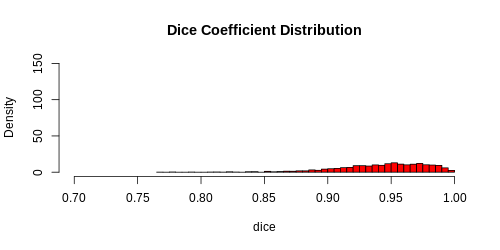
\includegraphics[width=.65\linewidth]{Figures/v1-val-dicedst-d.png}
    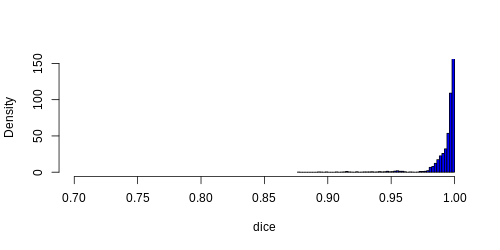
\includegraphics[width=.65\linewidth]{Figures/v1-val-dicedst-r.png}
    \caption{Dice coefficient distribution for the validation set - Initial Round}
    \label{fig:val-dice-dist}
\end{figure}

\begin{figure}[h!]
    \centering
    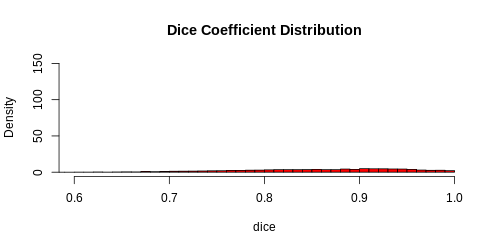
\includegraphics[width=.65\linewidth]{Figures/v2-val-dicedst-d.png}
    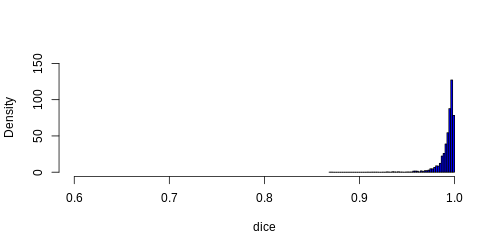
\includegraphics[width=.65\linewidth]{Figures/v2-val-dicedst-r.png}
    \caption{Dice coefficient distribution for the validation set - Improved Round}
    \label{fig:val-dice-dist-2}
\end{figure}

\begin{figure}[h!]
    \centering
    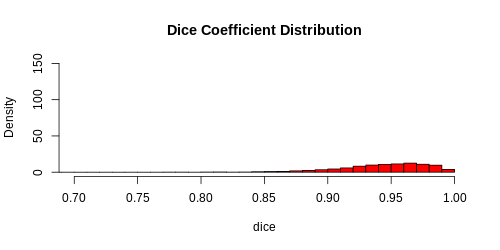
\includegraphics[width=.65\linewidth]{Figures/v1-tst-dicedst-d.png}
    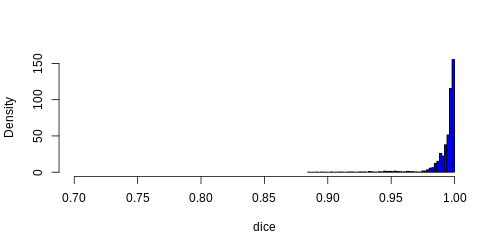
\includegraphics[width=.65\linewidth]{Figures/v1-tst-dicedst-r.png}
    \caption{Dice coefficient distribution for the test set - Initial Round}
    \label{fig:tst-dice-dist}
\end{figure}

\begin{figure}[h!]
    \centering
    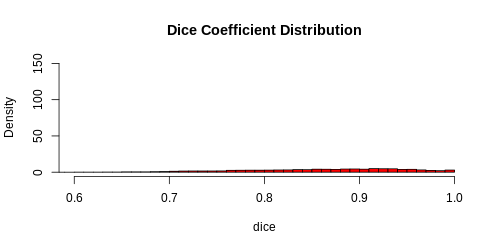
\includegraphics[width=.65\linewidth]{Figures/v2-tst-dicedst-d.png}
    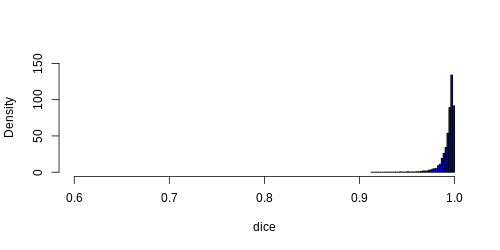
\includegraphics[width=.65\linewidth]{Figures/v2-tst-dicedst-r.png}
    \caption{Dice coefficient distribution for the test set - Improved Round}
    \label{fig:tst-dice-dist-2}
\end{figure}

\begin{figure}[h!]
    \centering
    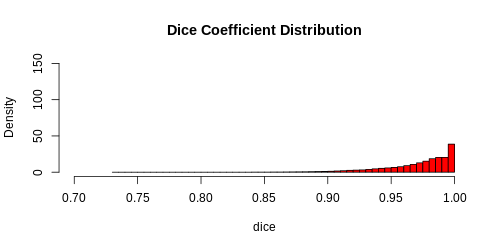
\includegraphics[width=.65\linewidth]{Figures/v2-mew2012-dicedst-d.png}
    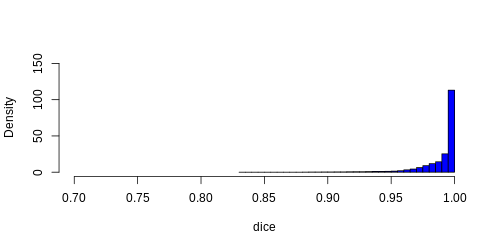
\includegraphics[width=.65\linewidth]{Figures/v2-mew2012-dicedst-r.png}
    \caption{Dice coefficient distribution for the MEW 2012 set}
    \label{fig:mew2012-dice-dist}
\end{figure}

In red, we plotted the dice coefficient comparing the damaged leaves with the original shapes, while in blue, we plotted the dice coefficient comparing the reconstructed leaves with the original shapes. The variances between the red and blue populations were different. Therefore, we chose to apply Welch's \textit{t}-test to compare the populations \cite{salkind2010encyclopedia}. For all studied cases, the \textit{p}-value was lower than $2.2 \times 10^{-16}$, indicating that the population means were not equal. In other words, the reconstruction process produced different shapes that were not caused by random events.

Regarding the reconstructed data, the average dice coefficient value for the validation set was 0.992 $\pm$ 0.008, while that for the test set was 0.993 $\pm$ 0.007. The worst-case values were 0.869 for the validation set and 0.912 for the test set. Finally, the average obtained from the MEW 2012 set was 0.988 $\pm$ 0.017.

\subsection{Technical Evaluation: How to embed this solution?}

In red, we plotted the dice coefficient comparing the damaged leaves with the original shapes, while in blue, we plotted the dice coefficient comparing the reconstructed leaves with the original shapes. The variances between the red and blue populations were different. Therefore, we chose to apply Welch's \textit{t}-test to compare the populations \cite{salkind2010encyclopedia}. For all studied cases, the \textit{p}-value was lower than $2.2 \times 10^{-16}$, indicating that the population means were not equal. In other words, the reconstruction process produced different shapes that were not caused by random events.

Regarding the reconstructed data, the average dice coefficient value for the validation set was 0.992 $\pm$ 0.008, while that for the test set was 0.993 $\pm$ 0.007. The worst-case values were 0.869 for the validation set and 0.912 for the test set. Finally, the average obtained from the MEW 2012 set was 0.988 $\pm$ 0.017.

\begin{enumerate}
    \item Interest region identification;
    \item Interest region segmentation;
    \item Image binarization.
\end{enumerate}

\begin{figure}[h!]
    \centering
    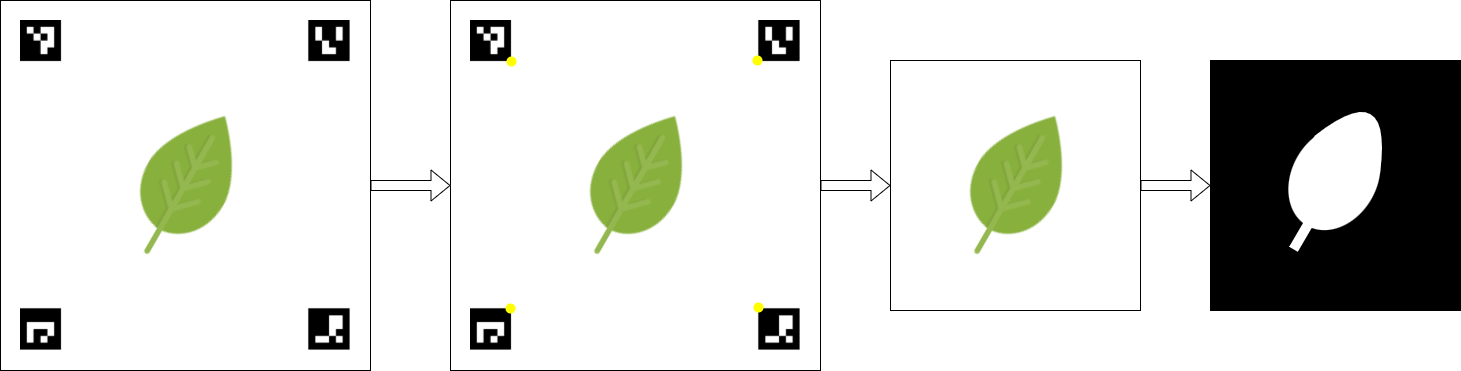
\includegraphics[width = \linewidth]{Figures/full-pipeline.png}
    \caption{Complete segmentation pipeline proposal}
    \label{fig:pipeline-proposal}
\end{figure}

The proposed pipeline is presented in Figure \ref{fig:pipeline-proposal}. The initial step in this process involves identifying the area where the user intends to place the leaf. This step is aided by the use of readily identifiable elements in the image, such as ArUco tags \cite{garrido2014automatic}. These tags are easily integrated into popular Computer Vision libraries and enable the identification of specific points. 

\begin{figure}[h!]
    \centering
    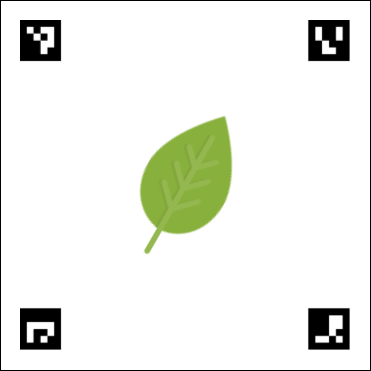
\includegraphics[width = .4\linewidth]{Figures/illustration.png}
    \caption{Illustration of the usage of ArUco tags to segment a map area.}
    \label{fig:illustration}
\end{figure}

We propose the use of four tags that delimit a square to aid in this process. The leaf should be positioned at the center of this square. This method helps to correct perspective issues that may arise due to camera tilt. An illustration of the proposed solution is presented in Figure \ref{fig:illustration}.

To segment the region, the algorithm must identify the four tags and extract the desired coordinates from each of them. Then, a perspective transformation is performed to convert the plane into a square. The expected results after this stage are displayed in Figure \ref{fig:stage-2}.

\begin{figure}[h!]
    \centering
    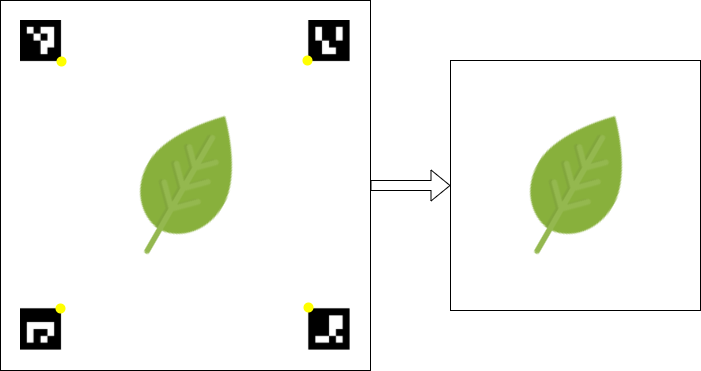
\includegraphics[width = .5\linewidth]{Figures/stage-2.png}
    \caption{Region segmentation process illustration}
    \label{fig:stage-2}
\end{figure}

After this stage, the algorithm obtains a square region with the leaf positioned above the background. At this point, we directly apply Otsu's binarization algorithm to the obtained segment. The expected result is displayed in Figure \ref{fig:stage-3}.

\begin{figure}[h!]
    \centering
    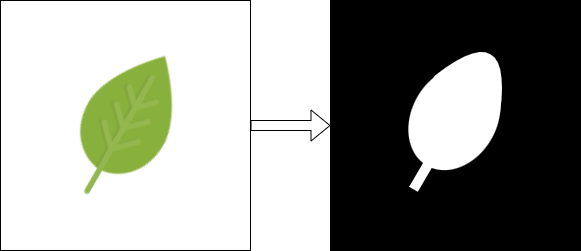
\includegraphics[width = .5\linewidth]{Figures/stage-3.png}
    \caption{Binarization process illustration}
    \label{fig:stage-3}
\end{figure}

We tested this pipeline under two different conditions. The first condition was a bench test. We produced the background according to the planned and provided a mockup leaf to test the segmentation process. Then, we also performed a small field test, in which we tried to capture and segment a leaf in the field using a camera and submitting it to this same process. Figure \ref{fig:experiments-final} displays the results for both tests. Our experiments displayed overall satisfactory results in both the bench and the field tests. The algorithm was able to segment the leaf from the background properly.

\begin{figure}[h!]
    \centering
    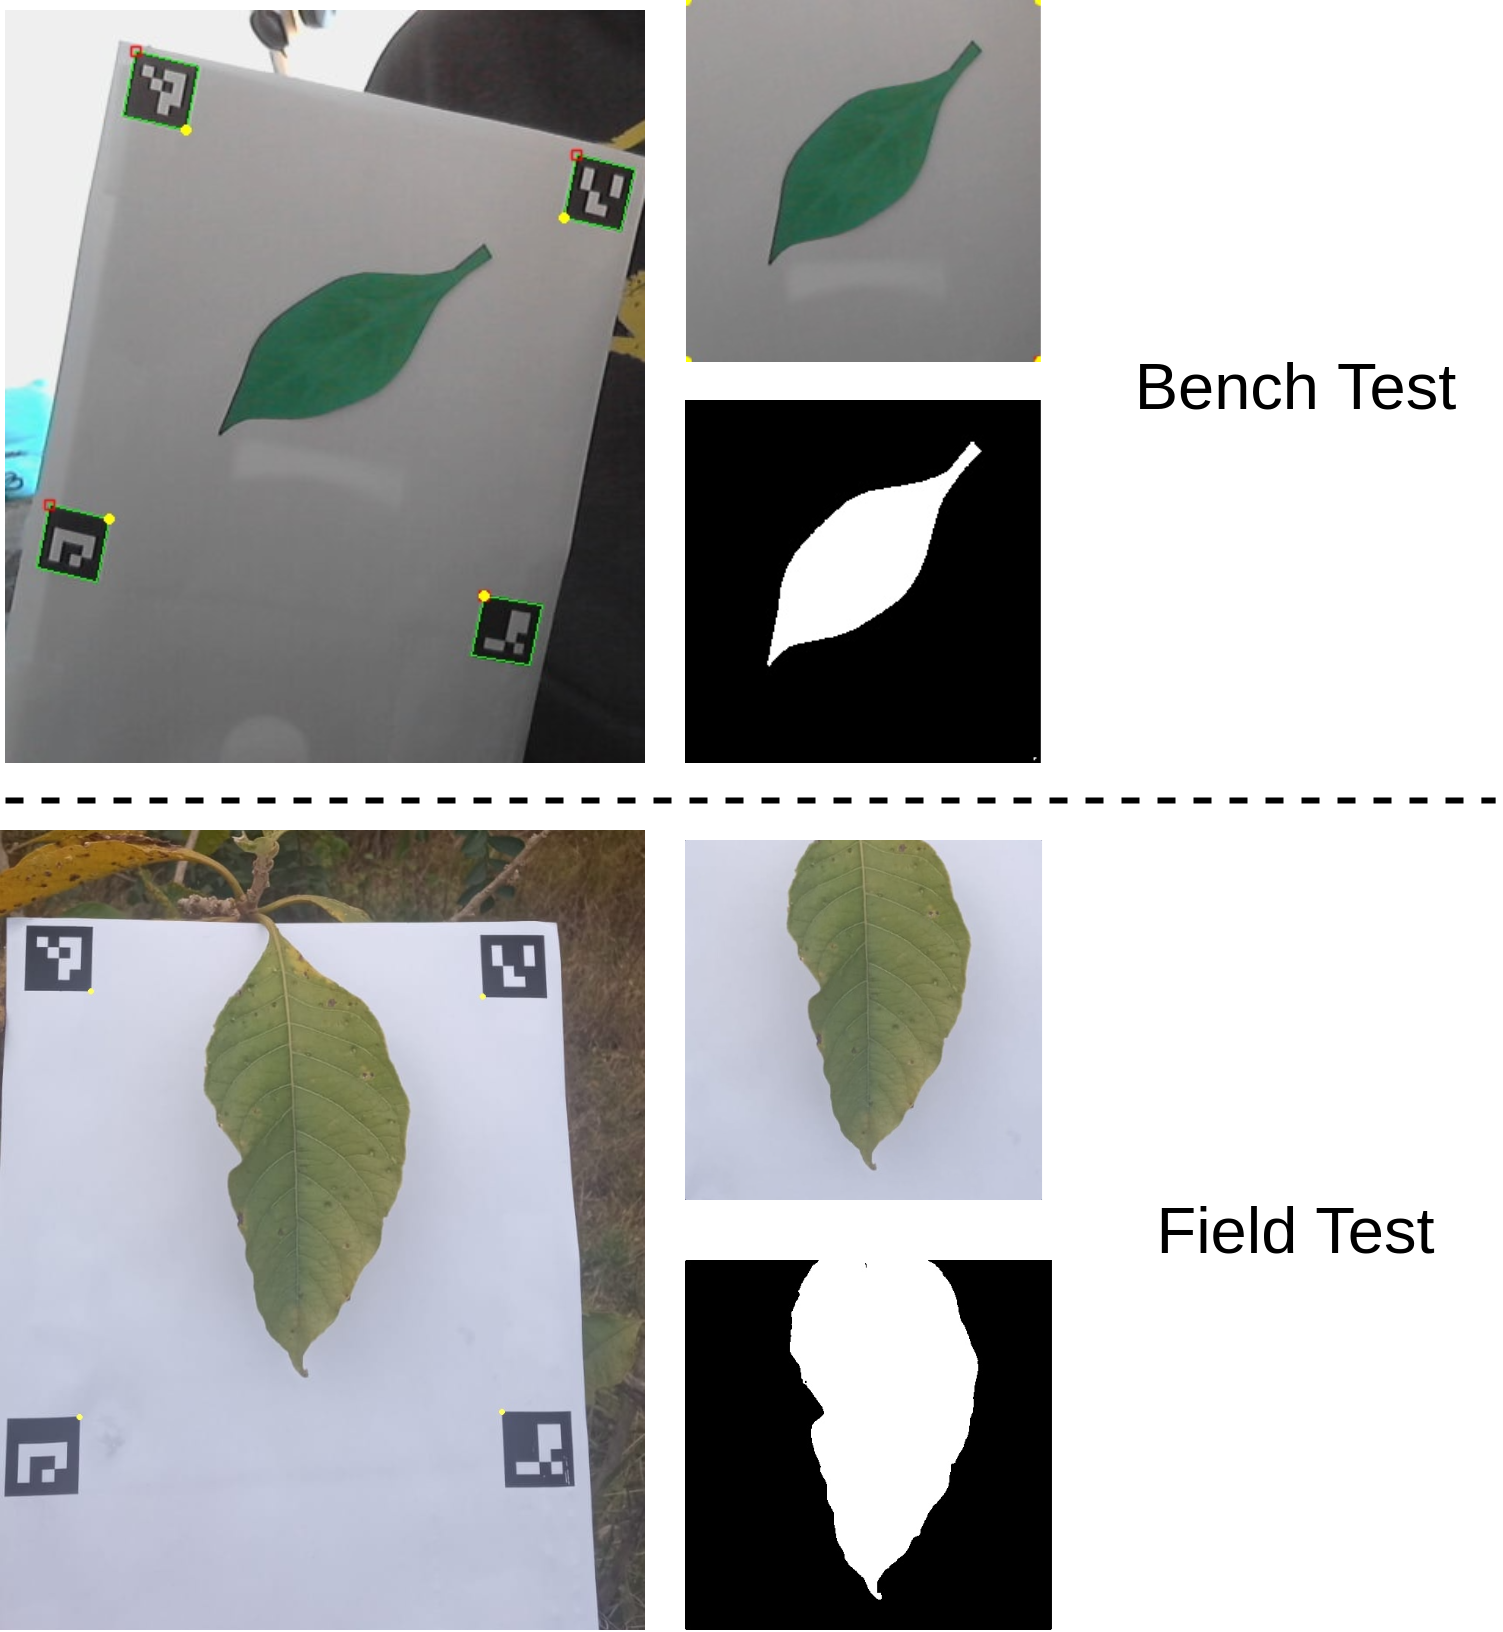
\includegraphics[width = .6\linewidth]{Figures/experiments.png}
    \caption{Experiments displaying the results of the proposed process. These experiments validate the usage of this technique to provide a mean to take this appliance onto the field.}
    \label{fig:experiments-final}
\end{figure}

%==========================================

\section{Evaluating and mapping diseases in forest canopies}

The case study involves a triangulation approach, where three individual climbers conducted a cylinder-transect investigation. This method is akin to the recommendation made by Ribeiro, Basset, and Kitching  \cite{ribeiro2014density} about density estimation. We employed this approach to develop the Edge AI system for identifying leaf diseases. The researchers initiate their approach by commencing at the highest point of the canopy and progressively descend downwards. They collect leaf samples along horizontal transects that are spaced at predetermined intervals until they reach the last stop. In this initial approach, to facilitate the division of data, we employ a backdrop template for sampling. The final destination is typically situated approximately 3 meters above ground level. The proposed methodology is depicted in Figure \ref{fig:cylinder}.

\begin{figure}[h]
    \centering
    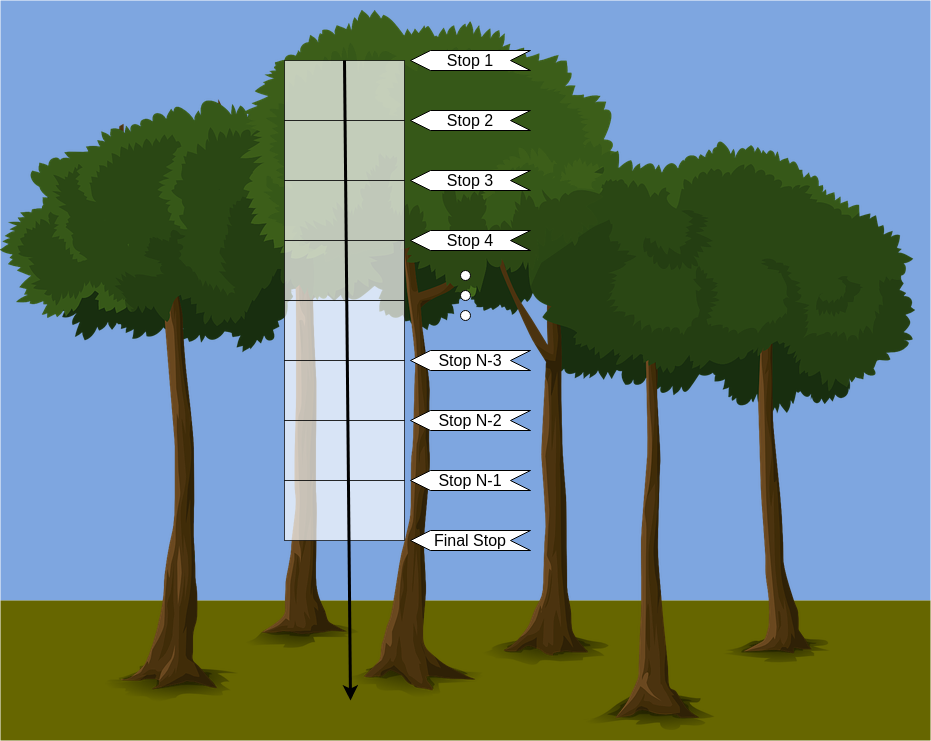
\includegraphics[width = .8\linewidth]{Figures/pin-cylinder.png}
    \caption{Illustration of the Cylinder-Transect study.}
    \label{fig:cylinder}
\end{figure}

Leaf conditions are highly significant markers of ecosystem health, as previously mentioned. García-Guzman et al. \cite{garcia2004incidence} demonstrated that in Mexican wet forests, the prevalence of diseased leaves can reach 65\% in highly infected areas, while it is only 2\% in locations with low infection rates. Given this baseline, we anticipate that the disease will be dispersed in both high and low infection locations whenever a pathogen is present in a canopy. From this viewpoint, we simulate the transmission of disease by utilizing a probability density function (PDF) that is centered on the location with the largest percentage of infected individuals. Figure \ref{fig:canopy-disease-spread} depicts a visual representation of a density gradient determined by a centered maximum.

\begin{figure}[h]
    \centering
    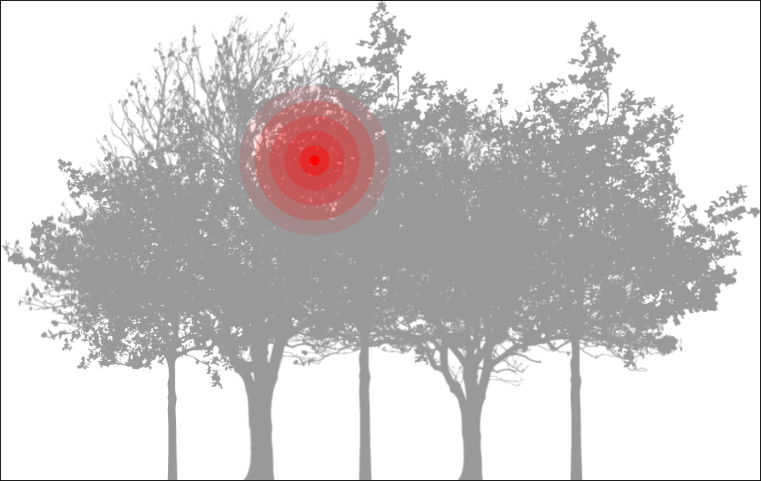
\includegraphics[width = .8\linewidth]{Figures/diseased-canopy.png}
    \caption{\color{black}Example of a possible location for a disease spread. We model this spread using a spatially-distributed probability density function (PDF).}
    \label{fig:canopy-disease-spread}
\end{figure}

We assume that the distribution is Gaussian in shape, extending across the canopy. Therefore, the distribution can be represented by a probability density function that follows a geometric function based on the Gaussian distribution. The function is expressed in Equation \ref{eq:pdf}. The function has the benefit of being able to represent the spread of the disease with only five parameters. The variable $p_0$ denotes the highest occurrence rate of the disease. The $\sigma$ parameter, as always, reflects the standard deviation. To simplify the analysis, we employed a uniform standard deviation across all three spatial dimensions. The $(x_0, y_0, z_0)$ coordinates represent the central point of the distribution. The objective of this work is not to delve into the intricacies of the modeling process, but rather to present a case-study that is straightforward and can be easily replicated.

\begin{equation}
\label{eq:pdf}
    P(x,y,z) = p_0 . e^{-\frac{(x-x_0)^2 + (y-y_0)^2 + (z-z_0)^2 }{2\sigma}}
\end{equation}

Several authors with prior experience in similar methodologies endorse the use of Gaussian-based models for disease transmission modeling. Soubeyrand, Enjalbert, and Sache \cite{soubeyrand2008accounting}  employed Gaussian-based modeling to simulate the circular diffusion of airborne plant disease. Pokharel and Deardon \cite{pokharel2016gaussian} conducted mathematical modeling of the transmission of infectious diseases using Gaussian distributions. In the midst of the COVID-19 pandemic, Ketu and Mishra \cite{ketu2021enhanced} utilized Gaussian-based models to forecast the spread of the disease.

Despite the existence of similar methods in the literature, we have selected this modeling approach over Gaussian random processes (GRPs) or Gaussian process estimators (GPEs) due to its distinct essential features, as highlighted by some of the writers. The authors Soubeyrand, Enjalbert, and Sache utilized GRPs in their suggested model, as outlined in their publication \cite{soubeyrand2008accounting}. The model involved the application of circular functions in a two-dimensional space to generate a preliminary representation. Our goal in this work is not to go into illness modeling. Therefore, we have chosen to develop a simplified model that relies on a single spatial function. Pokharel and Deardon \cite{pokharel2016gaussian} suggest employing Gaussian process approximations to construct emulators (GPEs) for a two-dimensional dynamic disease spread model. The objective differs in that the authors aim to incorporate additional variables and processes that are not the focus of this study.

Researchers employing the cylinder-transect approach in the canopy acquire the spatial arrangement of damaged and healthy leaves using established coordinates. While the depiction may appear uncomplicated, the process of doing a regression from density points in three-dimensional space to a continuous-space function is not straightforward. Therefore, we suggest employing a heuristic approach to acquire the parameters that more accurately depict the original function.

\subsection{Requirements}

To begin this study, it is necessary to assess the prerequisites for the proposed approach. To address this issue, we provide a modified version of the co-design diagram shown in Figure \ref{fig:simplified-codesign-2}, which is a simplified rendition of the diagram depicted in Figure \ref{fig:codesign-2.0}. 

\begin{figure}[ht!]
    \centering
    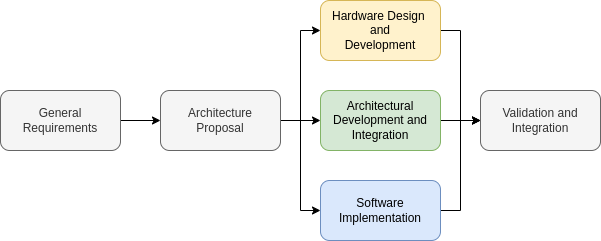
\includegraphics[width = .8\linewidth]{Figures/simplified-codesign.png}
    \caption{Simplified Co-design diagram.}
    \label{fig:simplified-codesign-2}
\end{figure}

This representation displays the need to raise the constraints for the application and classify them into the hardware, software or architectural domain. The constraints identified for this matter are:

\begin{itemize}
    \item As this system needs to be taken into the field, it needs to work for hours without a battery recharge or replacement. [\textit{Hardware}].
    \item It needs to be robust enough to take hits from branches and falling seeds or nuts. [\textit{Hardware}].
    \item As we propose a distributed system in a WBAN-Environment, both systems need to communicate with an application, working as web server nodes [\textit{Architecture}].
    \item The communication needs to be efficient to stream the data through this local network [\textit{Architecture}].
    \item The integrated architecture must present a mean to classify the leaves into diseased or healthy [\textit{Software}].
\end{itemize}

In this case, we proposed a cooperative wearable system in which several users can input gathered data into a local wireless server which provides the AI using its hardware acceleration. This system is able to run both a traditional machine learning method and a convolutional neural network, according to the available resources.

\subsection{General Architecture Proposal}

The suggested method utilizes a wearable distributed system that operates in both Wireless Body-Area Network (WBAN) and Wireless Local Area Networks (WLAN). This system is designed to enable the extraction of information using techniques such as Data Fusion, Image Processing, and Computer Vision. The provided diagram, labeled as Figure \ref{fig:architecture}, illustrates the suggested design for this system.

\begin{figure}[h!]
\centering
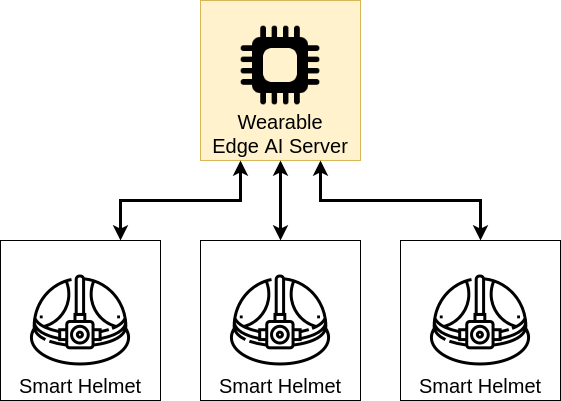
\includegraphics[width = .6\linewidth]{Figures/dataflow-2.png}
\caption{\label{fig:architecture}Proposed General Architecture. The smart helmets use the wearable Edge AI server to provide machine learning inferences.}
\end{figure}

The initial component of this system is the tangible nucleus. Since we are suggesting a wearable system, it is crucial that it is inconspicuous and does not cause any interference or disturbance \cite{bonato2003wearable}. Consequently, we constructed the system using hands-free technology for the user. The helmet is the optimal choice for meeting the wearable and research needs in terms of its physical core. The paper by Silva et al. \cite{silva2019toward} addressed the limitations imposed by certain appliances. Our main focus was to calculate the energy needs and usage for this particular system.

The subsequent component pertains to the fabrication of the sensor nodes that are based on the Internet of Things (IoT) technology. Every node is a Computer-on-Chip that has the ability to read sensor data, either single or numerous, process the data beforehand, and transmit it via either WBAN or WLAN. The selected sensors for enhancing environmental perception include a laser radar (LIDAR), a 9-Degree-of-Freedom Inertial Measurement Unit (9DoF IMU), and a conventional camera.

The Computer-on-Chip must possess the capability to access the necessary input/output ports from every sensor. Additionally, it is imperative that it possesses the capability to establish a wireless connection within the immediate vicinity of the body. Given the energy limitations of wearable systems, it is imperative that the Computer-on-Chip incorporates a processor with low power consumption. Therefore, ARM-based computer-on-chips are suitable solutions for this purpose. 

Typically, the preferred devices to serve as primary applications for this system are ARM-based Computer-on-Chips. These devices should include various I/O ports to connect the necessary sensors, as well as a network card that can transmit the data via a local wireless connection.

We choose the Wi-Fi network standard (IEEE 802.11) as the interface for our WLAN/WBAN. The decision was made considering the simplicity of developing web server solutions, the speed at which data can be transmitted, and the coverage area for WBAN/WLAN. Furthermore, it relied on the wider bandwidth capacity to ensure the quality of the connection, particularly while handling camera streaming. 

Each sensor node functions as a local webserver within this network. The application should explicitly request the sensor data from each node through the WBAN/WLAN. The application executes a data fusion technique. augments reality.

\subsubsection{Hardware Specification}

From the proposal, there are two main hardware element decisions: the \textit{Smart Helmet Hardware} and the \textit{Edge AI Node Hardware}.  In order to develop the intelligent helmet, we required a flexible and verified solution that includes a built-in camera. Conversely, the stage of selecting Edge AI Node Hardware must effectively balance performance and portability.

\paragraph{Smart Helmet Hardware}

This project is a progressive development of a wearable gadget designed for the purpose of studying and monitoring the ecological environment. Additional publications were authored by members of the research group, featuring findings that were previously examined. The articles \cite{silva2019toward, silva2019desenvolvimento} provide a detailed description of the hardware specification and its evaluation. The reproduction of the previously described evaluation is not the topic of this effort. Our objective is to include the suggested hardware into the Edge-AI architecture within this context.

This section offers a concise overview of the constructed wearable device and presents the necessary details and principles for the suggested integration. The hardware that has been created is a helmet consisting of sensors and a data processing unit. This tool was specifically designed for researchers and professionals who utilize the climb tree approach to gather data on natural habitats. 

\begin{figure}[ht]
\centering
\begin{subfigure}{.45\textwidth}
  \centering
  % include first image
  \includegraphics[width=\linewidth]{Figures/helmet2.JPG}  
  \caption{Assembled Wearable Device}
  \label{fig:proto}
\end{subfigure}
\begin{subfigure}{.45\textwidth}
  \centering
  % include second image
  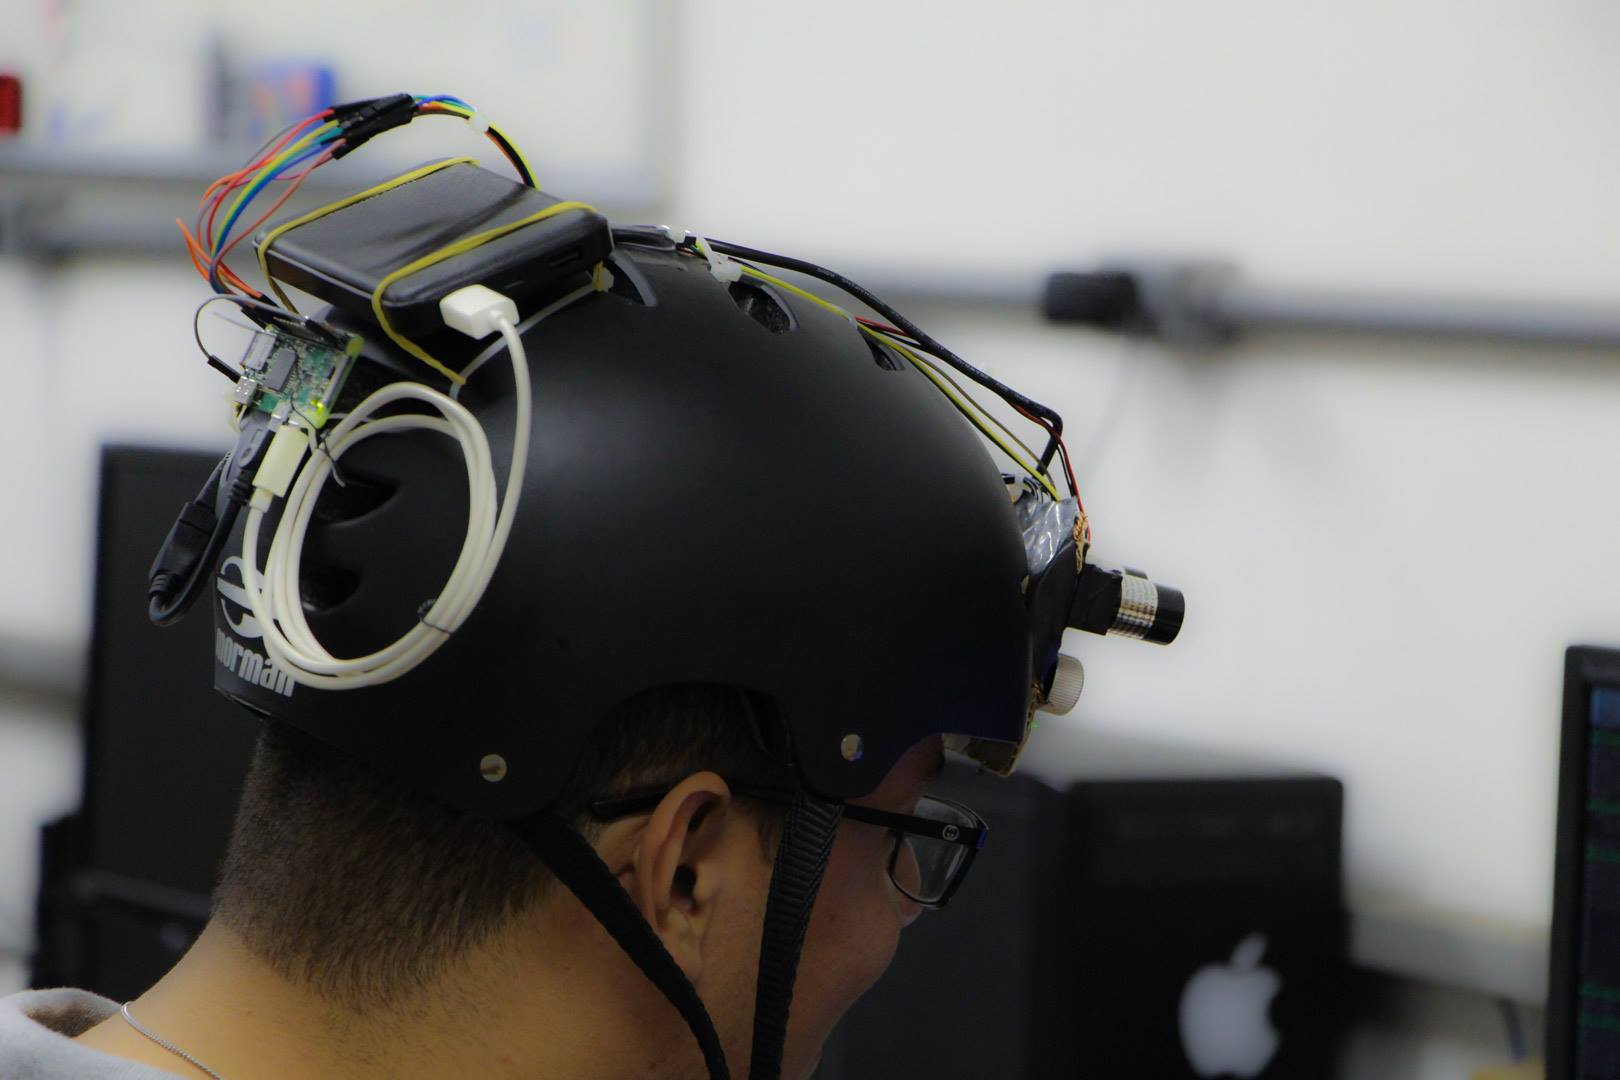
\includegraphics[width=\linewidth]{Figures/prototype2.jpg}  
  \caption{User wearing the device}
  \label{fig:wearing}
\end{subfigure}
\caption{Prototype Assembled}
\label{fig:Prototype}
\end{figure}

The wearable prototype is depicted in Figure~\ref{fig:Prototype}. Figure~\ref{fig:proto} displays a three-dimensional representation of the device, showing both the front and side views. Figure~\ref{fig:wearing} depicts a user wearing the device as seen from the rear. The hardware is equipped with a LIDAR sensor that is attached to a processing unit for accurately measuring the distance and estimating the 3D geometry of the objects being sensed. A Raspberry Pi Zero W was selected as the device for processing unit data, with power supplied by a 5V battery. During the development process, we took into account both the specifications for the wearable device and the needs for its use.

We utilized this prototype to do specific operations within this domain. Having already verified the sensing features of this system, our primary focus in this study was to conduct tests specifically evaluating its computational capability. Subsequent experiments have demonstrated that this prototype is capable of doing certain intended tasks, but its capabilities are restricted when confronted with more demanding processing requirements. Therefore, this viewpoint provides a rational basis for supporting the proposed Edge-based design. In the subsequent part, we will elaborate on the procedure of selecting the hardware for Edge Computing.

\paragraph{Edge AI server Node - Hardware selection and integration}

In addition to the smart helmet, another crucial component of the overall system is the Edge AI server node. Therefore, the hardware selection must take into account portable embedded systems that can facilitate machine-to-machine communication for this particular stage. Our case study focuses on implementing machine learning techniques within the setting of WBAN/WLAN to develop a viewpoint on Wearable Edge AI. This paper presents a comparison of the performance of four hardware components that have the capability to provide this utility.

\begin{figure}[h!]
    \centering
    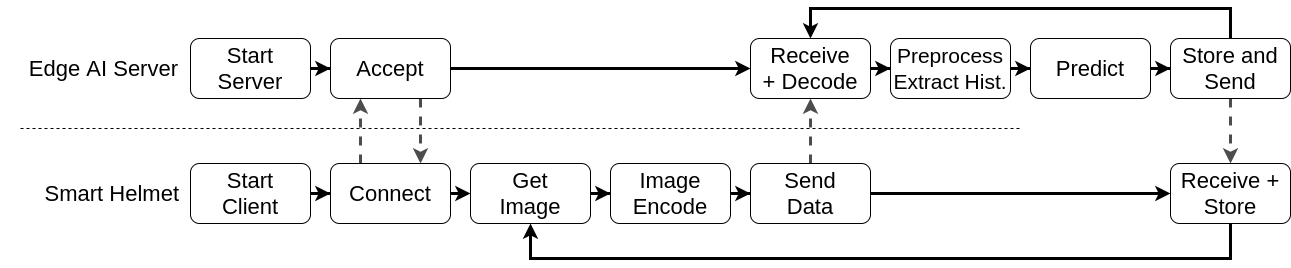
\includegraphics[width=\linewidth]{Figures/pipeline-Edge-AI.png}
    \caption{Edge AI service pipeline. In the proposed architecture, clients perform part of the processing, while the AI pipeline is provided by the Edge AI server node.}
    \label{fig:pipeline-edge-ai}
\end{figure}

Initially, we established a pipeline that separates the components which are processed locally from those processed within the Edge AI server node. At first, the local systems obtain and convert the image, transmitting the converted data to the edge server. Within this server, the application initializes a trained machine learning model and continuously receives encoded frames. It then proceeds to decode, preprocess, and extract the pseudospectrum from these frames, thereafter evaluating it. The assessment outcome is thereafter stored by the Edge AI server and returned to the device for duplication. The diagram in Figure \ref{fig:pipeline-edge-ai} illustrates the suggested pipeline for the Edge AI server, which is designed to accommodate a solitary client.

We evaluated multiple devices for developing the solution. In the context of this Wearable Edge AI solution, we evaluated the Raspberry Pi Zero W, Raspberry Pi 3B, Raspberry Pi 3B+, and Jetson Nano platforms as potential options for delivering Edge AI functionality. These solutions are all commercially available ARM-based computer-on-modules.

\subsubsection{Edge AI Software}

As stated in the introduction, the condition of leaves serves as crucial indicators of the overall health of the ecosystem. Therefore, we opted to assess the limitations of an Edge AI component that conducts leaf classifications into two categories: "normal" and "diseased." This section delves into the implementation of Edge AI software as demonstrated in the case study.

\begin{figure}[h!]
    \centering
    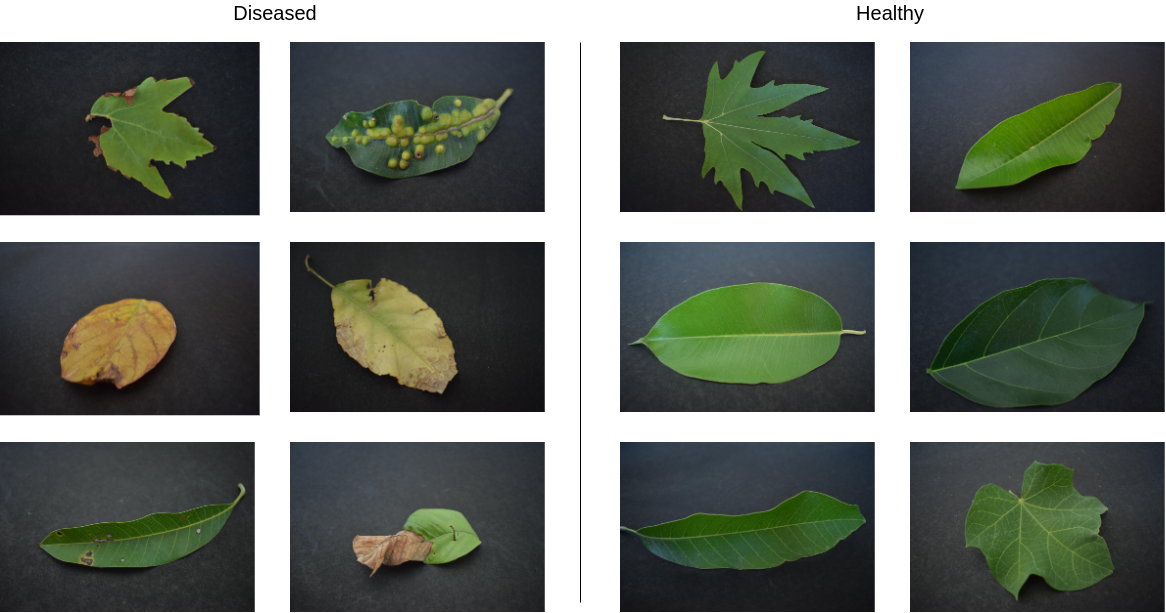
\includegraphics[width = .9\linewidth]{Figures/leaves.png}
    \caption{Sample of healthy and diseased leaf images obtained from the dataset.}
    \label{fig:healthy-and-diseased-leaves}
\end{figure}

\begin{figure}[h!]
    \centering
    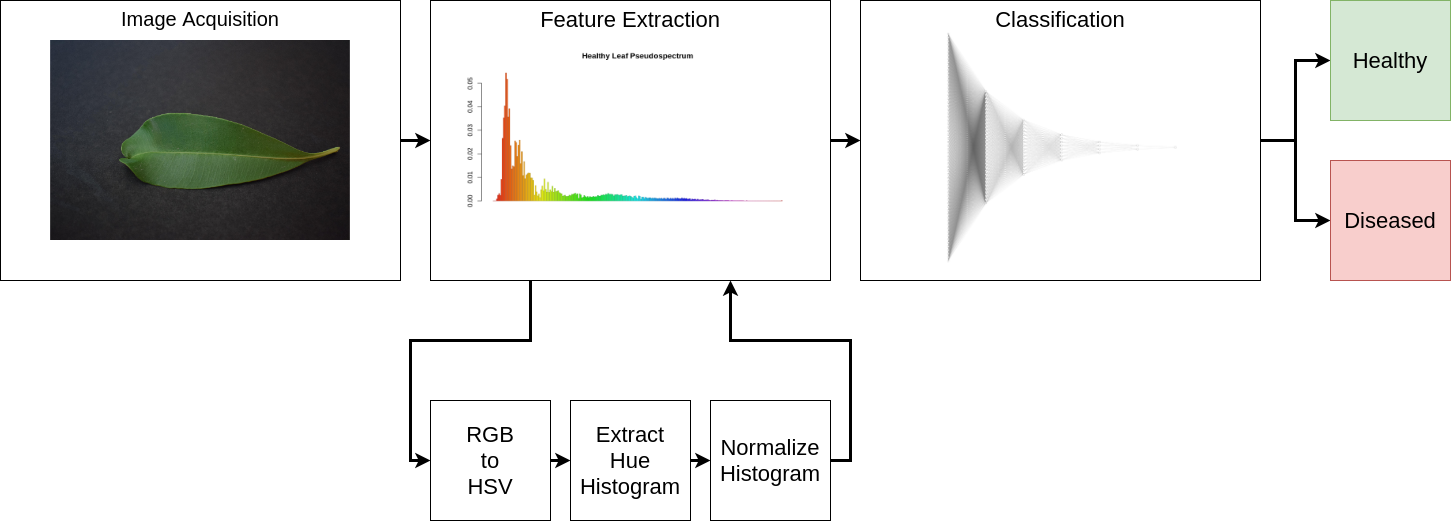
\includegraphics[width=.9\linewidth]{Figures/pipeline.png}
    \caption{Data processing pipeline and associated substages. For the image extraction, the associated stages are the color space conversion and histogram extraction.}
    \label{fig:pipeline}
\end{figure}

To begin, it is essential to locate a dataset that contains comparable information to the required dataset. After conducting thorough research, we have chosen to utilize the dataset provided by Chouhan, Kaul, and Singh in their publication on leaf diseases \cite{leaf-disease-dataset}. The authors provide a dataset consisting of 4,503 photos depicting leaves exhibiting both healthy and diseased conditions. Out of this collection, there are 2,278 photographs depicting healthy leaves, whereas 2,225 images show damaged leaves. There are 12 distinct species represented by the leaves. Figure \ref{fig:healthy-and-diseased-leaves} showcases photos of both healthy and diseased leaves extracted from the original dataset. 

The designers of this database ensure a clear distinction between infected and healthy leaves. Any variation in hue and texture is solely attributable to illness in all instances. The photos had a pixel resolution of 6,000x4,000. In order to enhance the test's speed and align the resolution with that of commonly used cameras in embedded systems, we reduced the resolution to 900x600 pixels. The improved resolution is equivalent to 15\% of the original size.
	
The data extraction and classification method adheres to a traditional pipeline. Initially, we obtain the image and then proceed to extract a feature vector. Next, we employ a machine learning model to categorize the image based on its attributes, resulting in a binary classification outcome. The pipeline is depicted in Figure \ref{fig:pipeline}, illustrating the substages linked to each primary stage.

\begin{figure}[h]
    \centering
    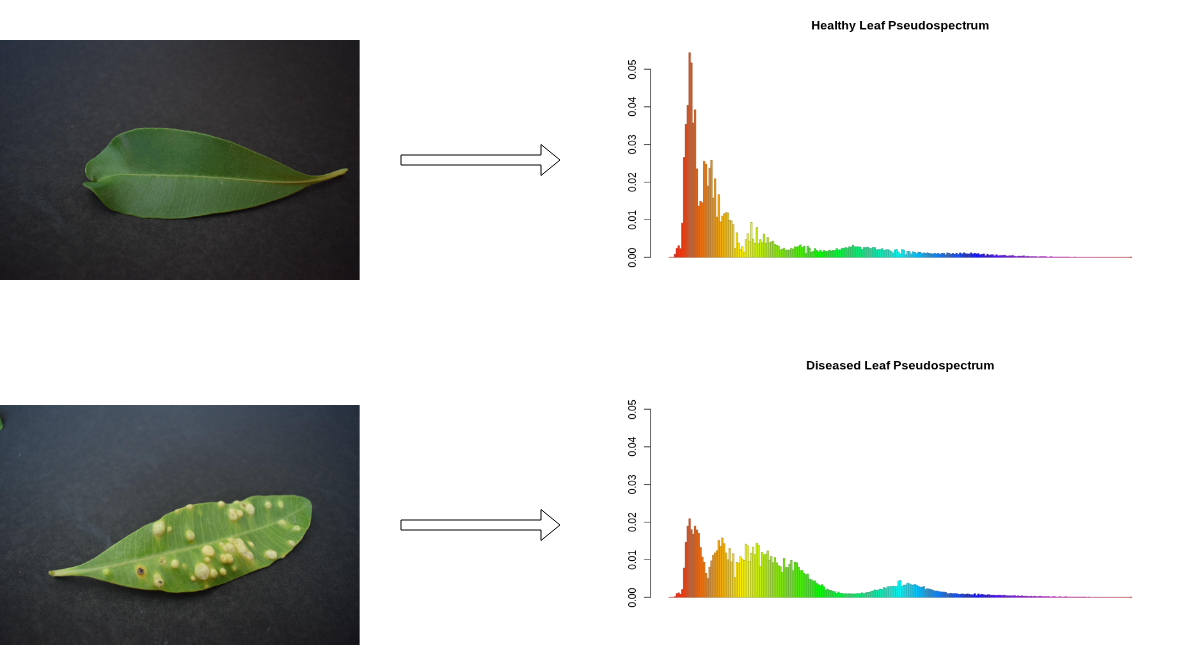
\includegraphics[width=.9\linewidth]{Figures/pseudospectrum-distribution.png}
    \caption{Pseudospectrum extraction samples}
    \label{fig:pseudospectrum}
\end{figure}

Within this particular framework, our method to addressing this issue involves the development of a pseudospectral analytic system \cite{iceis21orange}. In this process, the feature vector is a \textit{pseudospectrum}, which is obtained by extracting the histogram from the Hue channel in the HSV color space. Ultimately, the histogram is divided by its total sum, resulting in a probability density function (PDF) that represents the distribution of colors. This PDF is then referred to as the pseudospectrum. Figure \ref{fig:pseudospectrum} illustrates several instances of the extraction of pseudospectra.

\begin{figure}[h!]
    \centering
    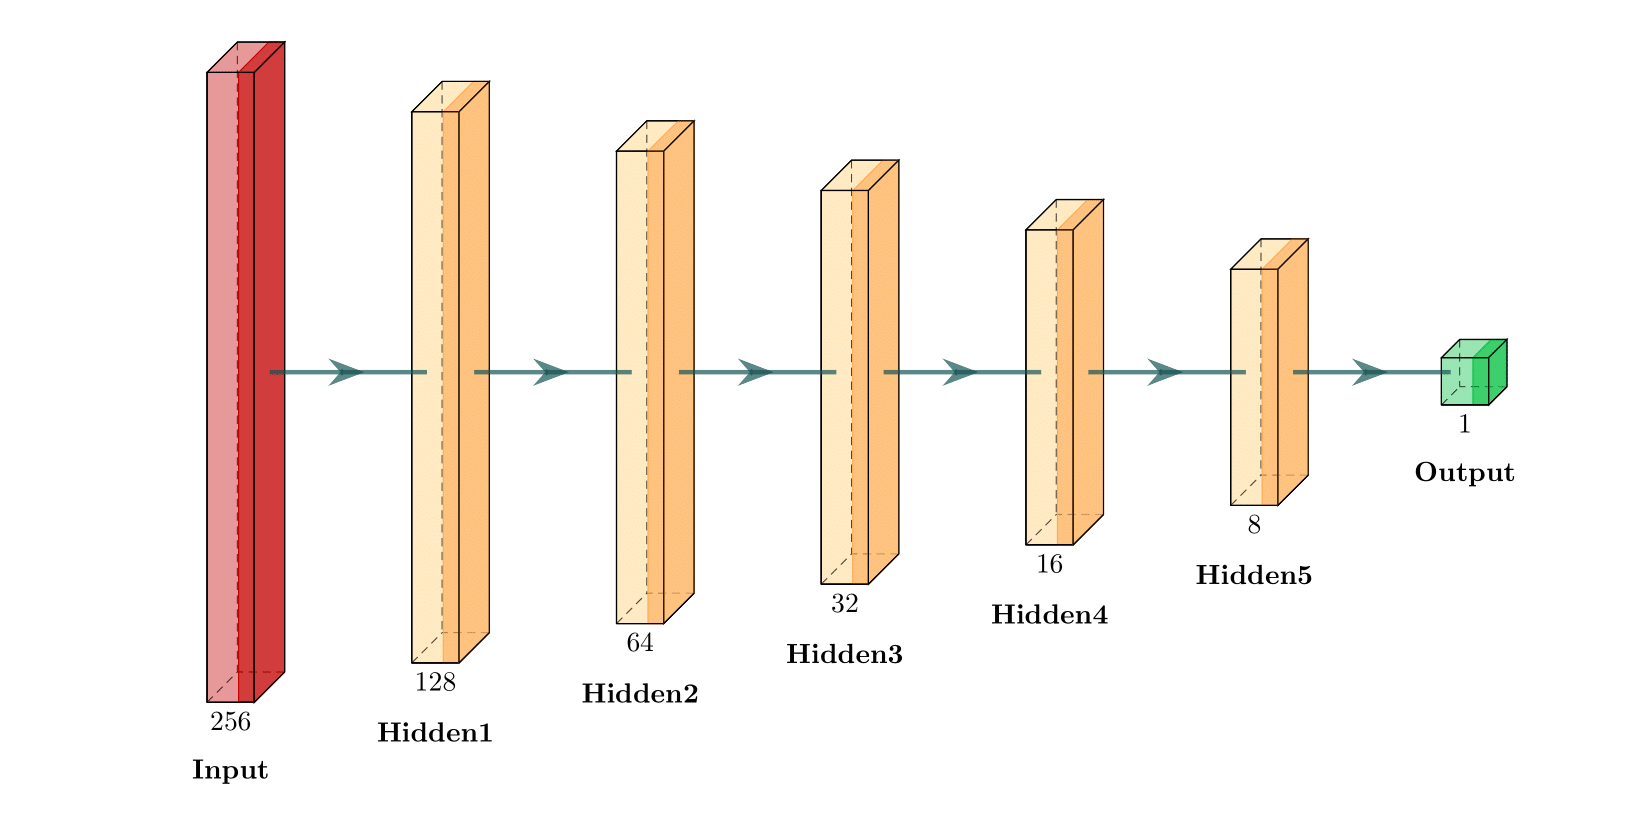
\includegraphics[width = .7\linewidth]{Figures/neuralnetwork-1.png}
    \caption{\color{black}Neural network representation. The chosen model was a Multi-Layer Perceptron (MLP). All layers are fully connected. The number beneath the blocks represents the number of neurons in each layer.}
    \label{fig:neural-network}
\end{figure}

Subsequently, a neural network is employed to categorize the leaf. In this instance, we employed a conventional Multi-Layer Perceptron (MLP) model to carry out the computations. Despite the model's lack of novelty, we selected it due to its simplicity, which results in improved performance on low-power devices in Edge Computing. Despite its simplicity, the model has demonstrated intriguing outcomes in the classification of citrus fruits \cite{iceis21orange}. Within this particular framework, we employed a network that received 256 inputs derived from the pseudospectrum. The network's hidden layers consisted of 128, 64, 32, 16, and 8 neurons, respectively. The result yielded a binary categorization of either healthy or diseased. Figure \ref{fig:neural-network} presents a concise representation of the network's structure.

\begin{figure}[h!]
    \centering
    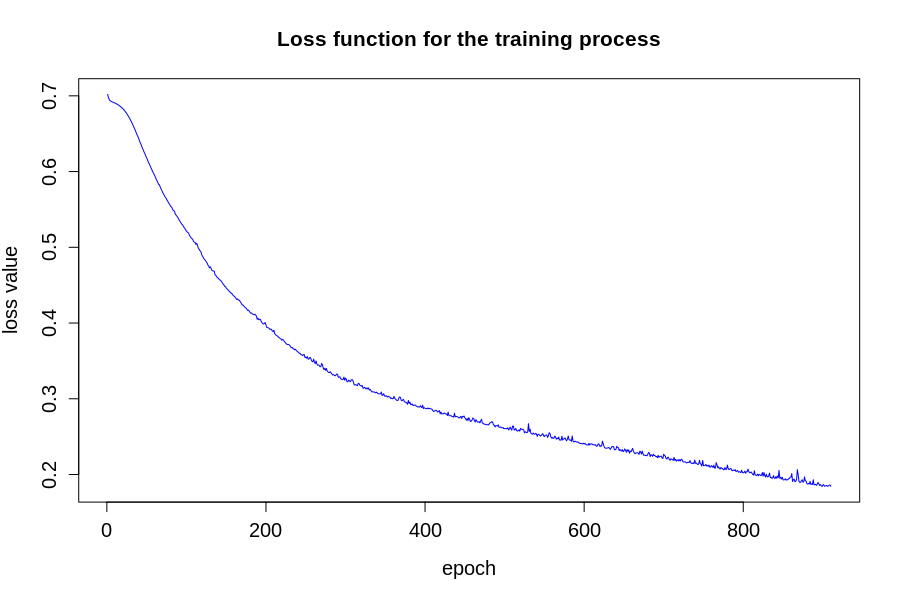
\includegraphics[width = .7\linewidth]{Figures/loss_function.png}
    \caption{Loss function during the training process}
    \label{fig:loss_function}
\end{figure}

The \textit{scikit-learn} framework was employed to construct our model \cite{pedregosa2011scikit}. The training was conducted using a backpropagation technique, employing a cross-entropy loss function. For the purpose of training, we partitioned the original dataset of photos into two distinct subsets. During the initial phase, we employed a random selection process to choose 10\% of the photos depicting both damaged and healthy leaves from each species. These selected images were then used to create a test dataset. The remaining 90\% constituted a training set. Our system was trained using 90\% of the photos from the training set, while the remaining 10\% were used for validation. The behavior of the cross-entropy loss during the training is depicted in Figure \ref{fig:loss_function}. This training concludes when the cross-entropy loss value does not improve by more than $10^{-5}$ for ten consecutive epochs, as determined by an arbitrary convergence criteria.

In addition to this model, we also evaluated the feasibility of utilizing a convolutional neural network (CNN) model for making predictions on the embedded hardware. This method is more contemporary, although necessitates a greater amount of computer capacity. Therefore, we put forward a test that assessed two aspects:


\begin{itemize}
    \item How much improvement can a CNN obtain over an Computer Vision and MLP.
    \item How much performance the embedded system loses using this method over a traditional approach.
\end{itemize}

We created a simple CNN model that approaches this process. Figure \ref{fig:CNN-model} displays an illustration of this model.

This model utilizes five 2D-convolutional layers in the feature extraction stage. The layers have 16, 32, 64, 64, and 64 filters of size 3x3, respectively. Following each convolutional layer, there is a further max pooling layer with a 2x2 size. Following these phases, the output is compressed and sent through a dense layer consisting of 1024 neurons. So far, the convolutional and dense layers have employed a rectified linear unit (ReLU) activation function. Ultimately, the result is a solitary neuron that utilizes a sigmoid activation function. The loss function employed was the cross-entropy. The function was trained for a total of 12 epochs, a value determined empirically as the maximum number of epochs to prevent overfitting indications. In addition, we conducted tests on this model based on the hardware and software performance indicators in order to address the problems that were highlighted.

\begin{figure}[h!]
    \centering
    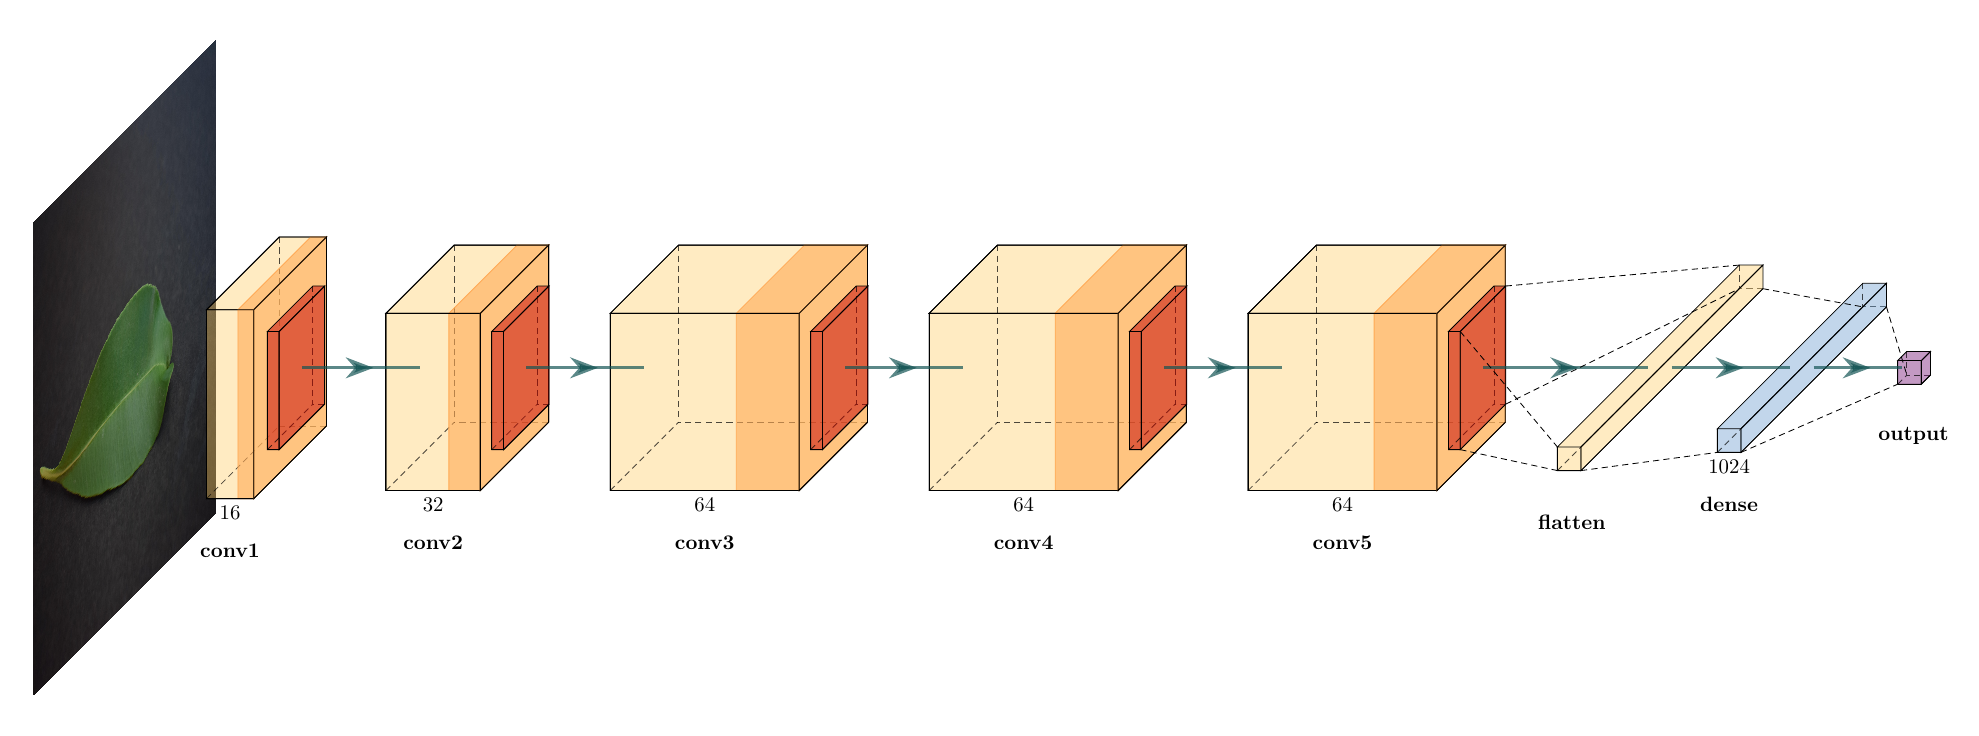
\includegraphics[width = \linewidth]{Figures/CNN_Sensors.png}
    \caption{Proposed CNN model. The convolutional layers have 3x3 filters, with 2x2 pooling. The output is a single value obtained from a sigmoid activation function.}
    \label{fig:CNN-model}
\end{figure}

\begin{figure}[h!]
    \centering
    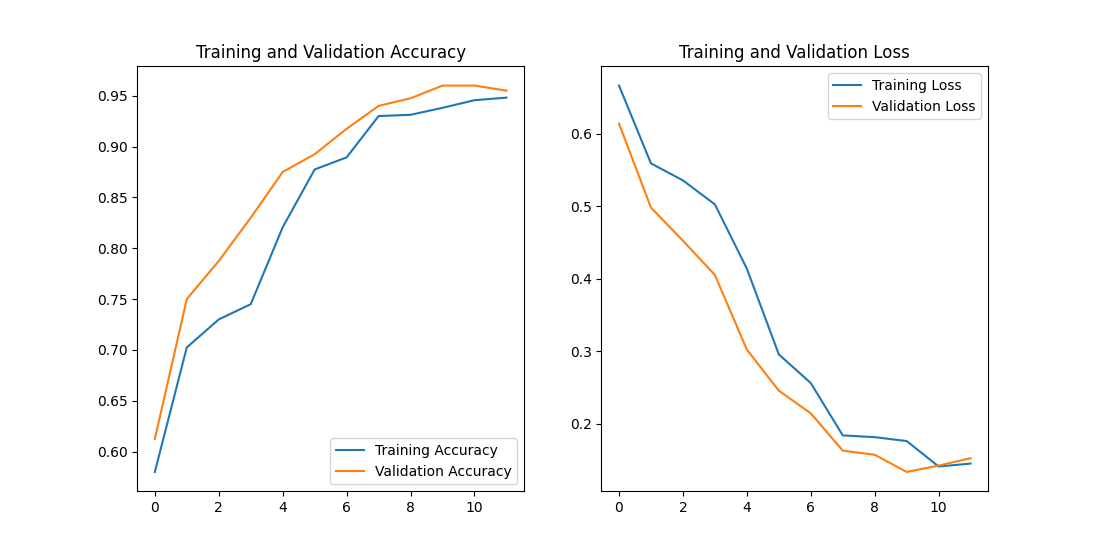
\includegraphics[width=\linewidth]{Figures/cnn_train_validation.png}
    \caption{Values for accuracy and loss functions in the CNN training process.}
    \label{fig:cnn-train}
\end{figure}

\subsection{Validation Tests}

Once we have put forth the hardware, software, and architectural components, it is essential to set metrics to verify the effectiveness of each stage. Within this area, we present the modeling and metrics utilized to assess each individual component. We assessed the performance of the Edge AI server across different platforms, focusing on the hardware components. We analyzed the metrics of the machine learning software predictions for the suggested application in order to evaluate its software features. Regarding the design, we analyzed the timing limitations for numerous clients linked to the Edge AI server, taking into account a Real-Time Quality of Service (QoS) assessment.

\subsubsection{Hardware Validation Tests}

This appliance consists of two primary hardware components: a Smart-Helmet and an Edge AI server node. The helmet was originally designed to provide versatile applications in this field. Hence, the validation stage deems it imperative to validate the newly introduced component: the Edge AI node. 

In Figure \ref{fig:pipeline-edge-ai}, we delineated the specific functions carried out by both the intelligent helmet and the Edge AI node. Initially, we must assess the hardware components for each of the recommended solutions based on the distributor websites associated with them. The available options include of the Raspberry Pi Zero W, Raspberry Pi 3B, Raspberry Pi 3B+, and Jetson Nano. Table \ref{tab:hardware-specs} presents the most relevant aspects about each solution.

\begin{table}[h!]
\centering
\caption{Hardware Specifications for the Edge AI server node candidates.}
\label{tab:hardware-specs}
\resizebox{\linewidth}{!}{%
\begin{tabular}{lllll}
\multicolumn{1}{l|}{} & \textbf{Raspberry Pi Zero W} & \textbf{Raspberry Pi 3B} & \textbf{Raspberry Pi 3B+} & \textbf{Nvidia Jetson Nano} \\ \hline \hline
\multicolumn{1}{l|}{\textbf{CPU}} & \begin{tabular}[c]{@{}l@{}}1x ARM11 \\ @ 1GHz\end{tabular} & \begin{tabular}[c]{@{}l@{}}4× ARM Cortex-A53 \\ @ 1.2GHz\end{tabular} & \begin{tabular}[c]{@{}l@{}}4× ARM Cortex-A53 \\ @ 1.4GHz\end{tabular} & \begin{tabular}[c]{@{}l@{}}4x ARM Cortex-A57\\ @ 1.43 GHz\end{tabular} \\ \hline
\multicolumn{1}{l|}{\textbf{RAM}} & 512 MB & 1GB & 1GB & 4GB \\ \hline
\multicolumn{1}{l|}{\textbf{Storage}} & MicroSD card & MicroSD card & MicroSD card & MicroSD card \\ \hline
\multicolumn{1}{l|}{\textbf{\begin{tabular}[c]{@{}l@{}}Nominal\\ Power\end{tabular}}} & \begin{tabular}[c]{@{}l@{}}5V over microUSB\\ (max. 6W)\end{tabular} & \begin{tabular}[c]{@{}l@{}}5V over microUSB\\ (max. 12.5W)\end{tabular} & \begin{tabular}[c]{@{}l@{}}5V over microUSB\\ (max. 12.5W)\end{tabular} & \begin{tabular}[c]{@{}l@{}}5V over P4 Jack Barrell\\ (max. 5W/20W modes)\end{tabular} \\ \hline
\multicolumn{1}{l|}{\textbf{\begin{tabular}[c]{@{}l@{}}Network\\ Platform\end{tabular}}} & 2.4GHz 802.11n & 2.4GHz 802.11n & \begin{tabular}[c]{@{}l@{}}2.4GHz/5GHz \\ 802.11b/g/n/ac\end{tabular} & \begin{tabular}[c]{@{}l@{}}2.4GHz \\ 802.11n \\ (over USB)\end{tabular}
\end{tabular}%
}
\end{table}

To conduct this test, we execute the tasks outlined in the pipeline depicted in Figure \ref{fig:pipeline-edge-ai} for every candidate. We assess the time delay required to complete all internal phases for each solution, executing identical code to receive input from a client, make predictions about the outcome (whether it is healthy or unhealthy), return the predictions, and store them in a text file. During the hardware evaluation, we just focus on the latency of the steps that are executed locally. The components of the system that rely on networking will be executed at a later time, taking into account the characteristics of the architecture. Additionally, we conducted a comparison of the two software techniques by testing the ratio of average predictions per second. This addresses one of the inquiries posed in the software proposal, namely evaluating the efficacy of the model on the embedded hardware.

\subsubsection{Software Validation Tests}

The unique software being presented is a machine learning-based prediction system that operates on an Edge AI server node. To address this issue, we utilized a Multilayer Perceptron (MLP) neural network model to accurately forecast whether leaf images exhibit signs of disease or are in a healthy state. Furthermore, we conducted an evaluation of the same measures for the CNN model in order to validate the enhancement in this characteristic by employing a more contemporary approach.

In order to successfully validate the program, it is imperative that we thoroughly comprehend the performance of this machine learning model in relation to the specific data at hand. Therefore, we employ conventional machine learning metrics to examine the data. We evaluate the confusion matrix, as well as the \textit{Precision}, \textit{Recall}, and \textit{F1-Score} metrics. The subsequent equations illustrate the formulas for various measures. The above equations define the variables as follows: $TP$ represents the count of true positives, $FP$ represents the count of false positives, $TN$ represents the count of true negatives, and $FN$ represents the count of false negatives.

\begin{equation} \label{eq1}
\begin{split}
Precision =  \frac{TP}{TP + FP} \\
\end{split}
\end{equation}

 \begin{equation} \label{eq2}
\begin{split}
Recall =  \frac{TP }{TP +FN} \\
\end{split}
\end{equation}

\begin{equation} \label{eq3}
\begin{split}
F1\text{-}Score = 2 \times \frac{Precision \times Recall}{Precision + Recall} \\
\end{split}
\end{equation}

\subsubsection{Architecture Validation Tests}

It is necessary to take into account characteristics that assess the individual and overall performance of the proposed scenario for the validation tests of the architecture. Therefore, we devised an experiment that was specifically designed as a Real-Time Quality of Service (QoS) test, drawing inspiration from previous research on IoT and Wireless Sensor Networks \cite{silva2019analyzing,iceis21dt}, with the aim of assessing the real-time constraint. This assessment assesses the proficiency in completing a series of tasks, taking into account both individual and network-related circumstances. 

At first, we consider duration as discrete intervals, as the set $D = d_i,  i \in \mathbb{N}$, where $d_{i+1} - d_i = \theta$, and $\theta$ is a constant sampling time. The soft real-time deadline will be represented by $\phi$, where $\phi = k \times \theta, k \in \mathbb{N}^*$. Thereby, we establish the following definitions:

\begin{definition} 
    Let $D = d_i$ be the finite set of nodes performing IoT-dependant tasks, where $i \in \mathbb{N}$;
\end{definition}

\begin{definition}
    Let $E = e_i$ be the finite set of events that each node performs, where $i \in \mathbb{N}$;
\end{definition}

\begin{definition}
    Let $L = l_{g,e}$ be the length of time interval that the node $g$ takes to perform an event $e$ during the execution, where $g \in G$ and $e \in E$;
\end{definition}

\begin{definition}
    Let $P = p_{i}$ be the set of patterns of events to be observed in the devices, where $p_i = E_i$, $E_i \subset E$ and $i \in \mathbb{N}$. In this case, all client devices will perform the same events in the same pattern;
\end{definition}

\begin{definition}
    Let $O = o_{i}$ be the finite set of observations of a certain pattern $p_i \in P$ on each device;
\end{definition}

The equation that represents the elapsed time $\lambda$ to observe a particular pattern $p_i \in P$ is:

\begin{equation}
    \lambda_{o_i} = \sum l_{g,e_k} | \forall e_k \in o_i, o_i = O_{p_i}
\end{equation}

All client devices in the network composition will have the same $\phi$ soft real-time deadline. Given this equation, let $\hat{O}$ be a subset of $O$, where $\lambda_{o_i} \leq \phi$, $\forall o_i \in \hat{O}$. Finally, given the sets $O$ and $\hat{O}$:

\begin{definition}
    Let $N$ be the number of elements on the set $O$;
\end{definition}

\begin{definition}
    Let $N_h$ be the number of elements on the subset $\hat{O}$;
\end{definition}

The quality factor $Q_f$ will be represented by the following equation:

\begin{equation}
    Q_f = \frac{N_h}{N} (\times 100 \%)
\end{equation}

This result represents how often the nodes execute a pattern of events without violating the soft real-time constraints. The clients represent the smart-helmets and will send data to the Edge AI server node in parallel on each test. 

\subsubsection{Case Study Validation for Deployment}

In order to verify the system in the case study, we employed a test that relied on the probability distribution function outlined in Equation \ref{eq:pdf}. The equation represents the likelihood of encountering damaged leaves during a sample procedure near the tree, as determined by the spatial coordinates. The function's maximum value is determined by the $P_0$ value, and the spatial location of the disease's epicenter is given by the $(x_0, y_0, z_0)$ coordinate. The situation is depicted in Figure \ref{fig:canopy-disease-spread}.

\begin{figure}[h!]
    \centering
    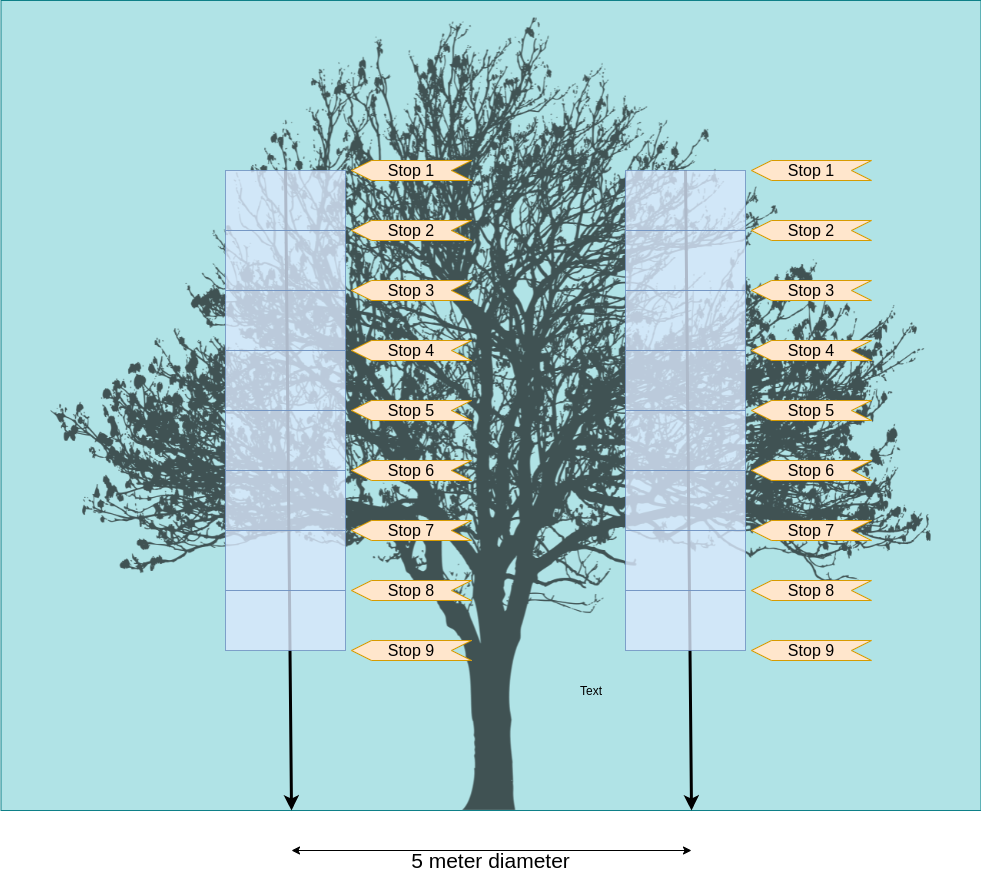
\includegraphics[width = .8\linewidth]{Figures/pin-cylinder-test.png}
    \caption{Sampling process illustration}
    \label{fig:pin-cylinder-test}
\end{figure}

For this validation test, we examine a group of three climbers who collect leaf samples at different heights inside certain areas of the canopy called transects. The whereabouts of the three climbers are arbitrary but known. Additionally, the locations of the stops along the transect are known, enabling the mapping of their positions as three-dimensional points during the procedure. The researchers should be positioned within a random radius from the center of the tree trunk in the canopy to achieve a more optimal spatial dispersion.  The organization for a 5-meter-radius and 9 stops is depicted in Figure \ref{fig:pin-cylinder-test}.

We examined a procedure that allows for an arbitrary number of stops during the ascent, in accordance with the requirements of the transect method. During each stop, the researcher would collect samples of leaf images. The system autonomously categorizes the sampled leaves as either healthy or unhealthy based on the acquired methodology. Consequently, for every $(x,y,z)$ coordinate at which a researcher employs the helmet and a backdrop template to sample the leaves, the system is capable of computing the proportion of unhealthy entities. 

For climbers to take tiny goods to the canopy, we suggest using a background template. This template is a sturdy object with identification tags placed along its edges. This suggestion enables the algorithm to circumvent any influence from the background during the sampling procedure. We created a preliminary examination to showcase this problem utilizing the wearable camera. The prototype captures the image, detects specific tags within the backdrop template, applies a four-point transformation to isolate the region of interest, and utilizes Otsu's binarization technique to segment the image. The pipeline utilized in this investigation is depicted in Figure \ref{fig:segmentation}.

\begin{figure}[h!]
    \centering
    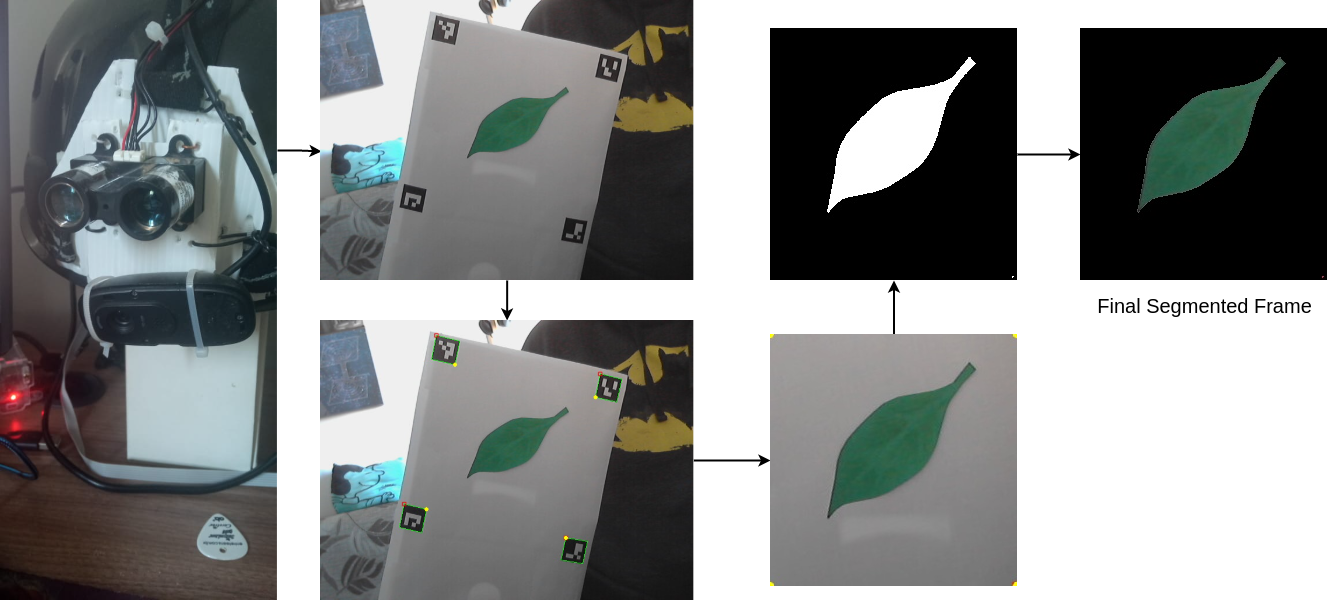
\includegraphics[width = .9\linewidth]{Figures/segmentation.png}
    \caption{Demonstration of the segmentation process. The prototype used a USB camera to capture the data, which can be processed by the prototype itself or in the Edge AI server node.}
    \label{fig:segmentation}
\end{figure}

Using this data, the system does a regression analysis to fit the probability density function (PDF) outlined in Equation \ref{eq:pdf}. To address this issue, it is necessary to acquire the parameters contained in the tuple $T = (p_0, \sigma, x_0, y_0, z_0)$. We opted to employ an Evolutionary Algorithm for the execution of this task, whereby the tuple candidates are regarded as the genotype and the mean squared error serves as the fitness function. {The decision was made considering three primary factors:}  

\begin{itemize}
    \item \textit{Ease of use:} it is easier to perform regression for a smooth parametric arbitrary three-dimensional distribution function with an evolutionary algorithm than designing an interpolation based in various parameters and kernel functions;
    \item \textit{Flexibility:} the same process can be used to obtain a regression to any parametric model by just changing the input parameters on the same algorithm;
    \item \textit{Robustness:} The regression algorithm displayed robust results, even with a change on its parameters.
\end{itemize}

In this case, the climbers would make nine stops, collecting 200 leaves at each stop. The system autonomously categorizes every leaf, transmitting data regarding each position and the compressed image of the leaf. To simulate the sampling process, we randomly selected 100 photos from the original dataset. Our selection approach utilizes a random number and evaluates its compatibility with the probability density function (PDF) defined by Equation \ref{eq:pdf} using arbitrary parameters. The value of $p_0$ was selected as $0.65$, taking into account the highest occurrence of sick leaves observed in the study conducted by García-Guzman et al. \cite{garcia2004incidence}. Furthermore, we established the coordinates of the tree stem and ground as the origin $(0,0,0)$ and deliberately chose $(2,-2,8)$ as the epicenter of the sickness. Ultimately, the value of our standard deviation ($\sigma$) was $5$. Therefore, the ultimate random PDF for this exam is:

\begin{equation}
\label{eq:arb-pdf}
    P(x,y,z) = 0.65 . e^{-\frac{(x-2)^2 + (y+2)^2 + (z-8)^2}{10}}
\end{equation}

Ultimately, the system categorizes and archives the data relative to the image. Our intention is to utilize the saved data to conduct an analysis that will yield the original PDF values through the implementation of an evolutionary algorithm. The Edge AI node is capable of conducting this analysis to offer on-site insights derived from the collected data. The goal is to approximate the original values of Equation \ref{eq:arb-pdf} as accurately as possible. Figure \ref{fig:arb_pdf} illustrates the spatial distribution of the disease in the given arbitrary function. The likelihood of encountering diseased leaves at this position increases as the red circle becomes larger and more vibrant in color. The brown stick denotes the location of the primary tree trunk.

\begin{figure}[h!]
    \centering
    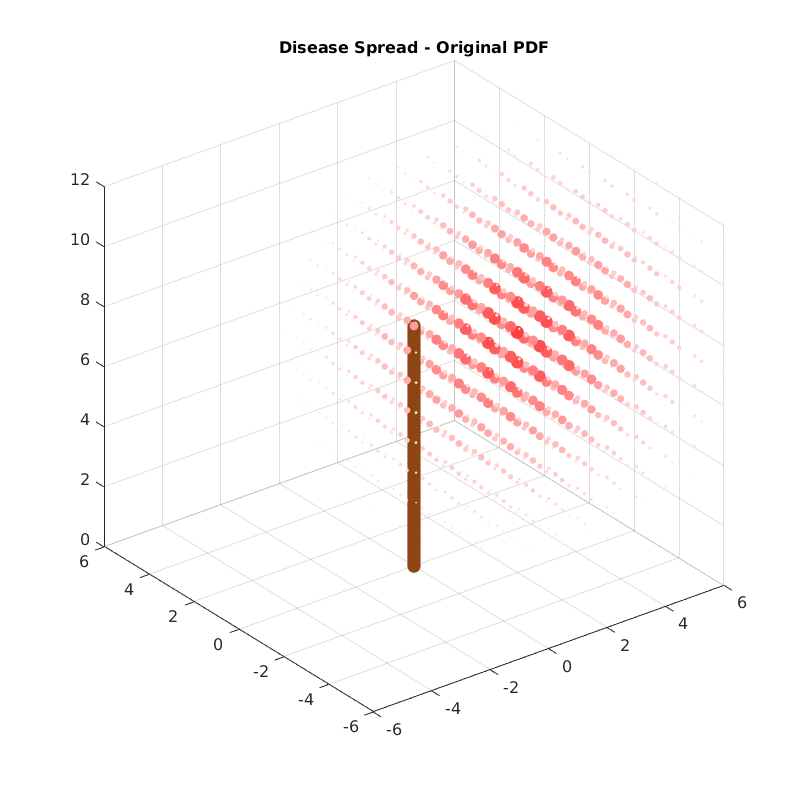
\includegraphics[width = .7\linewidth]{Figures/arb-pdf.png}
    \caption{Arbitrary PDF display. The larger and more colorful red dots have a bigger probability density. {\color{black}The brown cylinder represents the main tree trunk.}}
    \label{fig:arb_pdf}
\end{figure}

%%%%%%%%%%%%%%%%%%%%%%%%%%%%%%%%%%%%%%%%%%
\subsection{Results}

The preceding part provided a comprehensive overview of the hardware, software, and architecture components utilized in the proposed case study. In addition, we presented the assessment criteria employed to validate each branch of the co-design reviewed pattern. Ultimately, we deliberated on the verifications required for an application in the given case study. This section presents the results received from experiments conducted on the proposed elements.

\subsubsection{Hardware Validation Tests}

We present the hardware specifications for the Edge AI server node. All candidates are COTS computer-on-modules. To validate the hardware candidate, we assessed the candidates' performance in executing the internal Edge AI tasks. The pipeline for the proposed test is illustrated in Figure \ref{fig:hwtest-pipeline}. The internal duties for the Edge AI server are categorized into three stages: (i) preprocessing and extracting the feature vector, (ii) predicting the leaf condition, and (iii) storing the prediction data. 

\begin{figure}[h!]
    \centering
    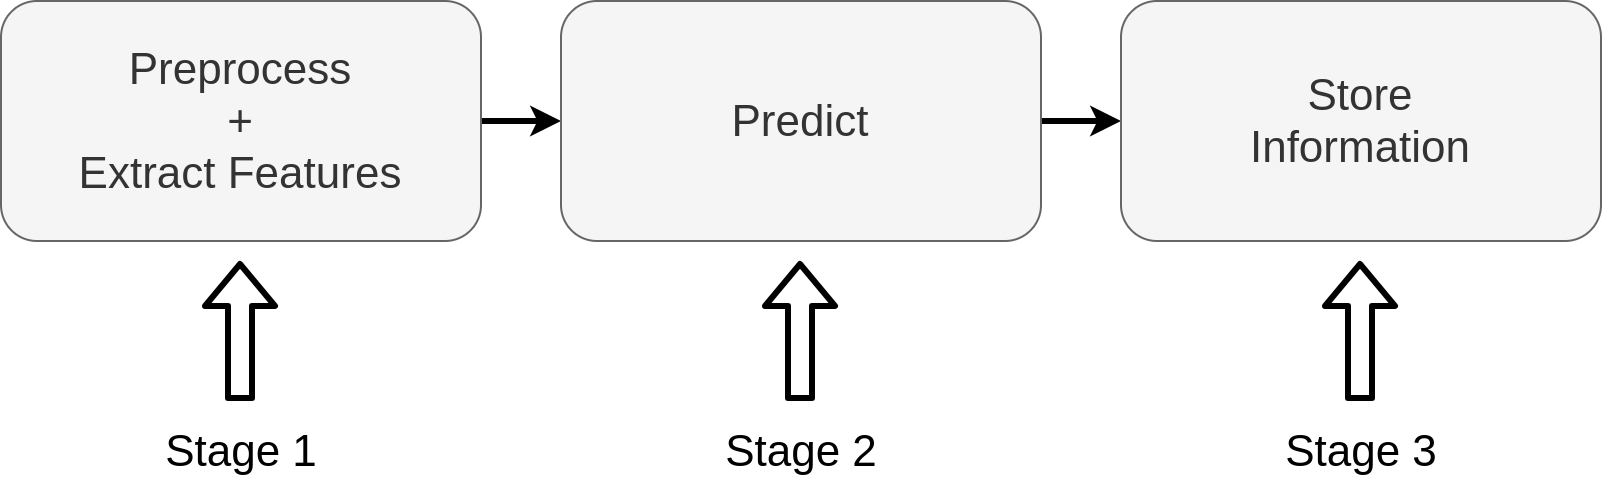
\includegraphics[width = .7\linewidth]{Figures/hw-test-pipeline.png}
    \caption{Pipeline for the hardware validation test.}
    \label{fig:hwtest-pipeline}
\end{figure}

We conducted the tests on all the candidates listed in Table \ref{tab:hardware-specs}. We conducted tests on the Jetson Nano in both the 5W and 20W power modes. We executed the subsequent pipeline on all 437 photos from the test set. The hardware candidates and configurations will be referred to as follows: \textit{Zero W} (Raspberry Pi Zero W), \textit{3B} (Raspberry Pi 3B), \textit{3B+} (Raspberry Pi 3B+), \textit{Jetson 5W} (Jetson Nano operating in 5W mode), and \textit{Jetson 20W} (Jetson Nano operating in 20W mode).

The Zero W was evaluated as it serves as the computer in the helmet prototype. The \textit{3B} and \textit{3B+} models were evaluated due to their lower pricing compared to the Jetson Nano, although having similar processor configurations. Using the \textit{Jetson 5W}, our goal is to compare the candidate with the highest cost but with limited hardware capabilities. In this economic operation mode, the operating system disables half of the CPU cores to conserve power. Ultimately, our objective was to confirm the disparity in performance between the priciest gear in the most powerful operational state and the performance of the other contenders.

\begin{figure}[h]
    \centering
    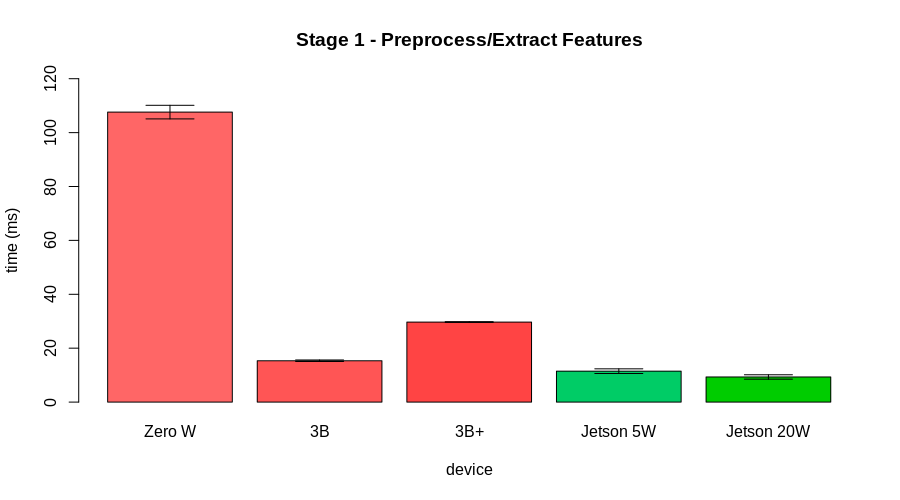
\includegraphics[width = .8\linewidth]{Figures/HW-stage1.png}
    \caption{Latency results for the first stage.}
    \label{fig:hw-stage1}
\end{figure}

Initially, we assessed the outcomes for Stage 1. During this stage, the hardware does preprocessing on the image by converting its color space from RGB to HSV. Next, it retrieves the pseudospectrum from the Hue channel. The latency evaluation findings from the first stage are presented in Figure \ref{fig:hw-stage1}. The \textit{Zero W} device completed the first stage in $107.61 \pm 2.53$ ms. The \textit{3B} device took $15.34 \pm 0.28$ ms to perform this task. The \textit{3B+} device took $29.69 \pm 0.13$ ms to complete this stage. The \textit{Jetson 5W} device took $11.47 \pm 0.87$ ms to perform this part, while the \textit{Jetson 20W} device took $9.32 \pm 0.81$ ms.

\begin{figure}[h]
    \centering
    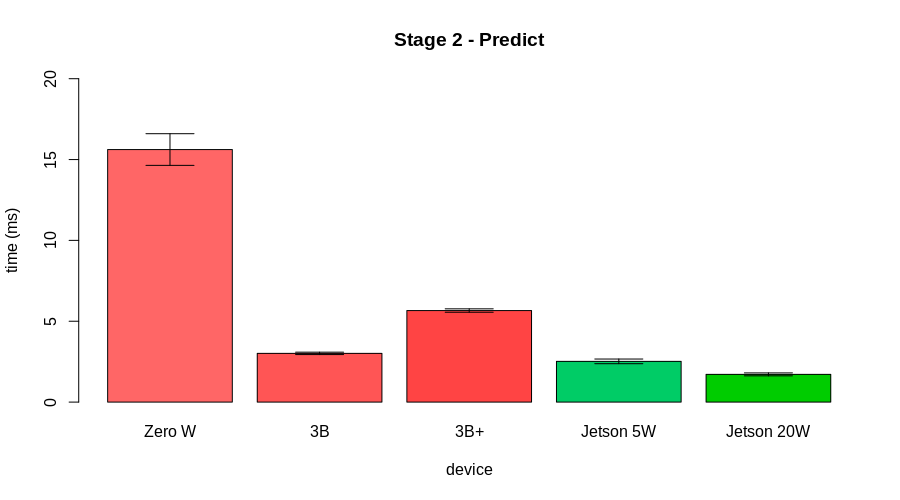
\includegraphics[width = .8\linewidth]{Figures/HW-stage2.png}
    \caption{Latency results for the second stage.}
    \label{fig:hw-stage2}
\end{figure}

Then, we assessed the results for the Stage 2. This stage corresponds to the prediction of the leaf condition using the model. Figure \ref{fig:hw-stage2} presents the results obtained from the evaluation of the latency from the second stage. \textit{Zero W} took $15.62 \pm 0.98$ ms to perform the first stage, \textit{3B} took $3.01 \pm 0.07$ ms to perform this task, \textit{3B+} took $5.66 \pm 0.10$ ms to perform this stage, \textit{Jetson 5W} took $2.52 \pm 0.14$ ms to perform this part, and \textit{Jetson 20W} took $1.71 \pm 0.09$ ms.

\begin{figure}[h]
    \centering
    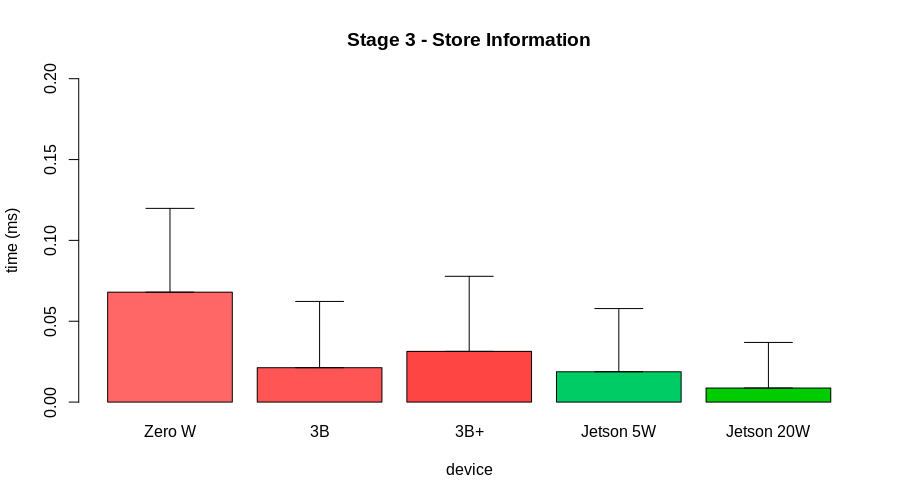
\includegraphics[width = .8\linewidth]{Figures/HW-stage3.png}
    \caption{Latency results for the third stage.}
    \label{fig:hw-stage3}
\end{figure}

At last, we analyzed the outcomes pertaining to Stage 3. This stage pertains to the retention of the information acquired from the preceding stages. The latency evaluation results from the second stage are depicted in Figure \ref{fig:hw-stage3}. The \textit{Zero W} required 0.07 ± 0.05 milliseconds to complete the initial stage. The \textit{3B} took 0.02 ± 0.04 milliseconds to accomplish this task. The \textit{3B+} required 0.03 ± 0.05 milliseconds to perform this stage. The \textit{Jetson 5W} took 0.02 ± 0.04 milliseconds to complete this part, whereas the \textit{Jetson 20W} took 0.01 ± 0.03 milliseconds. The observed discrepancies in this instance arose due to the time interval of this particular stage being shorter than the minimum recorded value, resulting in numerous measurements being conducted within an infinitesimally little timeframe.

All of the suggested gear is capable of executing the intended task. Therefore, the decision is made by assessing the performance, which may be subsequently compared to the project cost. Based on the test findings, it is evident that the Jetson Nano outperformed the Raspberry Pi 3B and 3B+ even when operating in power saving mode. The Raspberry Pi Zero W has the least amount of computational capacity, resulting in the poorest overall performance. Despite the similarities in hardware specs, the Raspberry Pi 3B outperformed the Raspberry Pi 3B+ and exhibited a performance level similar to the Jetson Nano operating in the 5W mode. The graph labeled as Figure \ref{fig:predpersec} illustrates the mean anticipated rate of predictions per second for each platform.

\begin{figure}[h]
    \centering
    \includegraphics[width = .8\linewidth]{Figures/predpersec.png}
    \caption{Average expected predictions per second ratio on each platform. The number in blue displays the expected ratio.}
    \label{fig:predpersec}
\end{figure}

As anticipated, the performance of the \textit{Zero W} was exceedingly poor. This supports the initial architectural idea to include an additional hardware component to handle the more demanding processing activities. Another anticipated outcome was the attainment of the highest level of performance using Jetson 20W. A notable finding is that, despite having a potentially superior processor, \textit{3B} exhibited significantly better performance than \textit{3B+}. Another significant finding is that despite disabling two out of the four cores, the \textit{Jetson 5W} exhibited higher performance compared to the \textit{3B} and \textit{3B+} models operating with all four cores and consuming over twice the amount of power. Given its ability to execute at a high level while operating under a power constraint, the \textit{Jetson 5W} is an excellent choice for field processing. Based on these findings, we conclude that \textit{3B} and \textit{Jetson 5W} are the primary contenders for fulfilling this application, as they exhibit the most favorable balance between performance and power consumption.

Ultimately, we assessed the ratio of average predictions per second by executing the CNN and MLP pipelines. The sole distinction in the CNN pipeline, as depicted in Figure \ref{fig:hwtest-pipeline}, is the absence of a feature extraction procedure, which is not necessary for the CNN. Therefore, this stage alone encompasses the alteration of input data to be provided to the model. The tests were conducted on the primary hardware options, namely Jetson 5W, Jetson 20W, and pi3B. The findings achieved for the predictions per second in the proposed setups were as follows:

\begin{itemize}
    \item The average predictions per second ratio in pi3B was $54 \pm 1$ for the MLP pipeline and $5 \pm 0$ for the CNN pipeline; \item The average predictions per second ratio in Jetson 5W was $71 \pm 5$ for the MLP pipeline and $10 \pm 0$ for the CNN pipeline;
    \item The average predictions per second ratio in Jetson 20W was $91 \pm 7$ for the MLP pipeline and $15 \pm 0$ for the CNN pipeline;
\end{itemize}

Figure \ref{fig:cnn-mlp-comp} also displays these results in the respective cited order. This data indicates that even in case of improvements on the software results, the CNN model is not adequate for time-restrictive tasks in the proposed configurations. This model is suitable to perform a later review of in-field captured results, but not to be integrated into a distributed constrained environment within the context of these tests.

\begin{figure}[h!]
    \centering
    \includegraphics[width = .32\linewidth]{Figures/pps-pi3B.png}
    \includegraphics[width = .32\linewidth]{Figures/pps-j5.png}
    \includegraphics[width = .32\linewidth]{Figures/pps-j20.png}
    \caption{MLP and CNN performance comparison test results.}
    \label{fig:cnn-mlp-comp}
\end{figure}

\subsubsection{Software Validation Tests}

The software validation tests in the previous section incorporate conventional ML metrics. Within this particular framework, we assessed the metrics of \textit{Precision}, \textit{Recall}, and \textit{F1-Score}. 

To ensure simplicity, the validation set is randomly selected from the training data only once. It contains 10\% of the total photos from the training data. The findings for the validation set are shown in Table \ref{tab:res-training}. The findings indicate that the system successfully detected the sick leaves in 90\% of the instances. Additionally, the Precision and Recall exhibit equilibrium, leading to a well-balanced F1-Score. This outcome suggests that the number of incorrect positive and negative results is almost equal. The confusion matrix obtained from this stage is displayed in Table \ref{tab:cfmat-valid}.

\begin{table}[h!]
\centering
\caption{Metric results for the validation dataset. This set was obtained separating 10\% of the training data for validation.}
\label{tab:res-training}
\resizebox{.6\linewidth}{!} \\ \hline
 & Precision & Recall & F1-Score & Support \\ \hline
healthy & 0.89 & 0.90 & 0.90 & 198 \\
diseased & 0.90 & 0.90 & 0.90 & 209 \\ \hline
\end{tabular}%
}
\end{table}

\begin{table}[h!]
\centering
\caption{Confusion Matrix for the validation data}
\label{tab:cfmat-valid}
\resizebox{.4\linewidth}{!}{%
\begin{tabular}{l|l|l|}
\cline{2-3}
 & \textbf{Healthy} & \textbf{Diseased} \\ \hline
\multicolumn{1}{|l|}{\textbf{Healthy}} & 178 & 20 \\ \hline
\multicolumn{1}{|l|}{\textbf{Diseased}} & 21 & 188 \\ \hline
\end{tabular}%
}
\end{table}

Additionally, we computed the global mean and the conventional metrics for the test dataset. Previously, the test set was partitioned by extracting 10\% of the photos from the original dataset. The acquired results for the validation set are shown in Table \ref{tab:res-test}, while the confusion matrix for this stage is displayed in Table \ref{tab:cfmat-test}. Once again, the results indicate that the system was able to accurately detect the sick leaves in approximately 90\% of the cases. Despite a slight disparity, the Precision and Recall exhibit equilibrium, leading to a harmonized F1-Score. This outcome validates the practicality of the suggested method within the specified framework.

\begin{table}[h!]
\centering
\caption{Metric results for the test dataset. This set previously separated, taking 10\% of all images.}
\label{tab:res-test}
\resizebox{.6\linewidth}{!} \\ \hline
 & Precision & Recall & F1-Score & Support \\ \hline
healthy & 0.93 & 0.88 & 0.91 & 217 \\
diseased & 0.89 & 0.93 & 0.91 & 220 \\ \hline
\end{tabular}%
}
\end{table}

\begin{table}[h!]
\centering
\caption{Confusion Matrix for the test data}
\label{tab:cfmat-test}
\resizebox{.4\linewidth}{!}{%
\begin{tabular}{l|l|l|}
\cline{2-3}
 & \textbf{Healthy} & \textbf{Diseased} \\ \hline
\multicolumn{1}{|l|}{\textbf{Healthy}} & 192 & 25 \\ \hline
\multicolumn{1}{|l|}{\textbf{Diseased}} & 15 & 205 \\ \hline
\end{tabular}%
}
\end{table}

Based on these stages, we can infer that the method is valid for the intended purpose. It accurately distinguishes between diseased and healthy leaves with an approximate accuracy of 90\%, and the outcomes are well-balanced. The following tests must verify the architectural characteristics of this solution. In addition, we conducted identical predictions taking into account the CNN. In this case, we utilized the identical test set to acquire the prediction outcomes.

\begin{table}[h!]
\centering
\caption{Metric results for the test dataset - CNN results. This set is the same previously separated for the MLP.}
\label{tab:res-test-cnn}
\resizebox{.6\linewidth}{!} \\ \hline
 & Precision & Recall & F1-Score & Support \\ \hline
healthy & 0.96 & 0.95 & 0.96 & 217 \\
diseased & 0.95 & 0.96 & 0.96 & 220 \\ \hline
\end{tabular}%
}
\end{table}

\begin{table}[h!]
\centering
\caption{Confusion Matrix for the test data - CNN results}
\label{tab:cfmat-test-cnn}
\resizebox{.4\linewidth}{!}{%
\begin{tabular}{l|l|l|}
\cline{2-3}
 & \textbf{Healthy} & \textbf{Diseased} \\ \hline
\multicolumn{1}{|l|}{\textbf{Healthy}} & 207 & 10 \\ \hline
\multicolumn{1}{|l|}{\textbf{Diseased}} & 9 & 211 \\ \hline
\end{tabular}%
}
\end{table}

As expected, the CNN performed better than the MLP. The results exhibit a 5\% enhancement in precision compared to the previous results. This outcome reinforces the necessity of utilizing this approach in future investigations instead of the MLP model. From the standpoint of leveraging greater processing capacity for data analysis, the Convolutional Neural Network (CNN) is a more favorable model compared to the Multilayer Perceptron (MLP).

\subsubsection{Architecture Validation Tests}

The architecture validation test assesses the capacity to execute a task while adhering to a soft real-time limitation. It refers to a performance assessment that offers a comprehensive perspective of the scalability of the suggested architecture. In this case, we employed the Jetson Nano as an Edge AI server to execute the pipeline illustrated in Figure \ref{fig:pipeline-edge-ai}. We designed a version of this system for the client that gives latency statistics for the steps marked in Figure \ref{fig:archtest-dataflow}.

\begin{figure}[h!]
    \centering
    \includegraphics[width = .9\linewidth]{Figures/archtest-dataflow.png}
    \caption{Stages considered in the architectural validation test.}
    \label{fig:archtest-dataflow}
\end{figure}

All clients have access to a uniform set of events. The number of nodes executing the tasks is equivalent to the number of devices carrying out the IoT-dependent operations. This experiment involves augmenting the client count and assessing its impact on the soft real-time restriction.

Thus, it is necessary to initially assess the real-time criteria in relation to the pipeline depicted in Figure \ref{fig:archtest-dataflow}. Therefore, we conducted the test taking into account the latency of the procedures for a solitary customer. Additionally, the test takes into account a series of finite discrete time intervals. Within this framework, we have designated the smallest time interval as 1 millisecond. The delay for each step in a single-client test is shown in Figure \ref{fig:arch-steps-latency}. In order to establish the soft real-time constraint ($\phi$), we assessed the minimum quantity of blocks required to deliver the service to a single client with a 100\% level of quality ($Qf = 1.0$), along with an extra 10\% allowance for loosening the criterion. We established the value of $\phi$ as 90 milliseconds using this approach.

\begin{figure}[h!]
    \centering
    \includegraphics[width = .8\linewidth]{Figures/arch-steps-latency.png}
    \caption{Latency for each of the steps presented in Figure \ref{fig:archtest-dataflow}}
    \label{fig:arch-steps-latency}
\end{figure}

Once $\phi$ was defined, we conducted multiple iterations of the test with 2 to 9 clients, all of whom were assigned the same assignment. The simulations were conducted on a computer machine that was linked to the WLAN network, serving as the Edge Server. During each test, every instance executed the identical test described in Figure \ref{fig:archtest-dataflow}, measuring the duration of each desired occurrence. Ultimately, we calculated the average and standard deviation of the quality factor, taking into account all the nodes that were part of the analysis. The test result is shown in Figure \ref{fig:qf-result}. This outcome demonstrates that the performance of the Edge-AI service deteriorates as the number of customers increases, while adhering to a specific real-time limitation. However, the system maintains a high level of quality despite having a small number of connected clients.

\begin{figure}[h!]
    \centering
    \includegraphics[width = .8\linewidth]{Figures/qf-test.png}
    \caption{Quality Factor test result}
    \label{fig:qf-result}
\end{figure}

Ultimately, we must ascertain whether the degradation in quality was a result of server overload or if other factors had an impact on the simulation program. In this regard, we quantified the mean latency of each stage while progressively increasing the number of nodes. Although steps one and two are contingent on the specific device being used, step three is vulnerable to potential network congestion, and the success of step four hinges on the efficiency of the Edge AI node. The findings for this analysis are displayed in Figures \ref{fig:latency-result-1}, \ref{fig:latency-result-2}, \ref{fig:latency-result-3}, and \ref{fig:latency-result-4}.

As anticipated, the latency in the initial two stages remained unaffected by the growing number of customers. These steps rely solely on the client carrying out its tasks. The third step introduces the initial action that relies on the network. The growing clientele may pose a challenge in the communication process. The findings indicate that this excessive load leads to an increase in delay for this particular stage, albeit the effect on the ultimate outcome is negligible (about 2 milliseconds). Ultimately, stage 4 reveals that the excessive burden on the Edge AI node is the primary element contributing to a decline in quality as the number of clients increases. This level is associated with both networking and the process of machine learning inference.

\begin{figure}[h!]
    \centering
    \includegraphics[width = .8\linewidth]{Figures/latency-st1.png}
    \caption{Latency test results for step 1}
    \label{fig:latency-result-1}
\end{figure}

\begin{figure}[h!]
    \centering
    \includegraphics[width = .8\linewidth]{Figures/latency-st2.png}
    \caption{Latency test results for step 2}
    \label{fig:latency-result-2}
\end{figure}

\begin{figure}[h!]
    \centering
    \includegraphics[width = .8\linewidth]{Figures/latency-st3.png}
    \caption{Latency test results for step 3}
    \label{fig:latency-result-3}
\end{figure}

\begin{figure}[h!]
    \centering
    \includegraphics[width = .8\linewidth]{Figures/latency-st4.png}
    \caption{Latency test results for step 4}
    \label{fig:latency-result-4}
\end{figure}


\subsubsection{Case Study Validation for Deployment}

We additionally conducted a validation phase for the entire solution. To address this issue, we created a simulation based on a case study appliance to test the proposed approach. Within this application, a trio of researchers employ the cylinder approach to sample 200 leaves at various predetermined heights. The Edge AI server node use predictive algorithms to determine the status of each leaf and subsequently records this information alongside the corresponding researcher coordinates. The researchers are positioned within a circular area with a diameter of 5 meters around the tree trunk in this device. Figure \ref{fig:solution-organization} illustrates the arrangement of various devices in relation to the tree trunk.

\begin{figure}[h!]
    \centering
    \includegraphics[width = .7\linewidth]{Figures/case-study-geometry.png}
    \caption{Upper view of the case study organization}
    \label{fig:solution-organization}
\end{figure}

We utilized Equation \ref{eq:arb-pdf} as the reference point for randomly choosing leaves from the sets of infected and healthy samples. Initially, the probability baseline was determined by computing the $(x,y,z)$ coordinate of each researcher at the given position. Subsequently, the computer creates a random number within the interval of $[0,1)$ for each of the 200 samples. If the value is below the baseline probability, the algorithm will choose a diseased leaf. Alternatively, it chooses a nutritious one.

\begin{figure}[h!]
    \centering
    \includegraphics[width = .6\linewidth]{Figures/sampled-disease.png}
    \caption{Case Study sampling distribution. {\color{black}The larger and more colorful red dots have a bigger percentage of diseased leaves. The brown cylinder represents the main tree trunk.}}
    \label{fig:sampling-result}
\end{figure}

After this process, we performed a test with the trained model. The test program uses each sample to estimate the leaf conditions for every device and location. Using this dataset, the application computes the proportion of infected leaves, resulting in a distribution sample. The outcomes of the sampling procedure are depicted in Figure \ref{fig:sampling-result}, taking into account the organization shown in Figure \ref{fig:organization}. As depicted in Figure \ref{fig:arb_pdf}, there is a positive correlation between the size and color intensity of the red dots and the prevalence of diseased leaves.

\begin{figure}[h!]
    \centering
    \includegraphics[width = .6\linewidth]{Figures/regression-pdf.png}
    \caption{Estimated PDF display. The larger and more colorful red dots have a bigger probability density. {\color{black}The brown cylinder represents the main tree trunk.}}
    \label{fig:comparison-pdf}
\end{figure}

Finally, we used an evolutionary algorithm to perform a regression to the parametric PDF presented in Equation \ref{eq:pdf} using the sampled data. Some features of this algorithm are:

\begin{itemize}
    \item Each individual genotype is a $T = (p_0, \sigma, x_0, y_0, z_0)$ tuple;
    \item The population has 100 individuals;
    \item Each round generates 70 offspring (30\% elitism);
    \item Each round has a complementary local search in half the population;
    \item The algorithm stops with a convergence criteria and RMSE lower than 0.05 (5\%);
\end{itemize}

To understand how good would a prediction be, we ran the model 20 times, and evaluated the average value for each paramenter of the $T = (p_0, \sigma, x_0, y_0, z_0)$ obtained from the best individual of the population. The average responses obtained from this experiment are:

\begin{itemize}
    \item $p_0 = 0.65 \pm 0.03$. The original value was $0.65$.
    \item $\sigma = 12 \pm 0.86$. The original value was $5$.
    \item $x_0 = 1.96 \pm 0.21$. The original value was $2$.
    \item $y_0 = -1.52 \pm 0.35$. The original value was $-2$.
    \item $z_0 = 8.1 \pm 0.16$. The original value was $8$.
\end{itemize}

The estimated spatial distribution of the disease based on these factors is shown in Figure \ref{fig:comparison-pdf}. The obtained values closely align with the anticipated outcomes. The distance between the predicted epicenter of the disease and the original PDF is 0.48 meters. The greatest predicted percentage closely approximates the original value. The variability of the predicted model is greater than that of the original module. The variation in results can be attributed to the inherent uncertainty of the leaf categorization model, which is approximately 10\%. Despite the prevailing ambiguity, the model yielded a reliable estimation for the parameters of disease propagation, based on the collected data. We conducted experiments by manipulating the algorithm's parameters to determine if the resulting outcomes would be altered. The findings of our study indicate that variations in population size, number of offspring, and maximum epochs had a negligible effect on the outcomes. This outcome demonstrates the high level of resilience in the process of acquiring the model parameters.

\section{Ant distribution and counting estimation}

Comprehending the actions of groups of ants is a crucial obstacle in the field of ecology. Helanterä et al. \cite{helantera2009unicolonial} assert that unicolonial ant populations are the largest cooperative units in nature. According to them, these species are able to construct extensive, interconnected nests. Furthermore, the authors assert that researchers in this domain can generate valuable data by understanding the dynamics of these colonies.

McGlynn \cite{mcglynn2012ecology} states that insect colonies are mobile entities, moving nests through their lifetime. The authors assert that understanding the factors that influence the mobility of the researched species requires knowledge of several aspects, such as its genetics, life-history evolution, and the effect of competition. Specifically, the authors assert that ant migration patterns are often unclear.

Regarding the methods of understanding the migration patterns of ant colonies, Hakkala et al. \cite{hakala2019evolution} state that reliable data capture of the colony motion is needed. Furthermore, they assert that by integrating this data with environmental information, it is feasible to understand how the setting influenced their migration. Technology solutions serve as a method to improve data collection and develop creative solutions for this issue.

Majer and Heterick \cite{majer2018planning} also evaluate the subject of devising experiments to achieve this objective. According to the authors, prolonged observation is crucial for doing research on invertebrates. This element also ensures that the development of innovative technology instruments aimed at this objective has a favorable impact on researchers in this field.

This study investigates the development of an innovative instrument that enables researchers to assess the dynamics within ant colonies. Our anticipation is to utilize the developed technology to derive data pertaining to quantities and distribution. Our objective was to develop an automated system capable of quantifying the number of ants in the solution. The solution also enables an assessment of the approximate distribution of the ants inside the scene.

\subsection{Requirements}

The first step in this analysis is evaluating the requirements for the proposed method. For this matter, we display a version of the co-design diagram presented in Figure \ref{fig:simplified-codesign-3}, which is a simplification of the diagram presented in Figure \ref{fig:codesign-2.0}. 

\begin{figure}[ht!]
    \centering
    \includegraphics[width = .8\linewidth]{Figures/simplified-codesign.png}
    \caption{Simplified Co-design diagram.}
    \label{fig:simplified-codesign-3}
\end{figure}

This picture illustrates the necessity of increasing the limitations for the application and categorizing them into the domains of hardware, software, or architecture. The limits identified for this matter are as follows:

\begin{itemize}
    \item This system must use lower-processing CNNs to match embedded edge server devices [\textit{Hardware}].
    \item This system must be able to approach how many ants are present in a scene and estimate a spatial distribution. [\textit{Software}].
    \item The application must use similar validated tools to allow its integration into a cooperative schema [\textit{Architecture}].
\end{itemize}

In order to address this issue, we decided to conduct experiments using various Convolutional Neural Networks (CNNs) that have limited memory and processing requirements. The purpose of these experiments is to take a partially quantitative approach to assessing the significance and dispersion of ants. A crucial element of this concept is the attainment of the hardware restriction through a software design.

\subsection{{Methods overview}}

In the preceding sections, we evaluated the significance and originality of the proposed solution. There is no previous example in the literature of a similar solution being produced. Within this part, we delve into the intricacies of the suggested resolution. We thoroughly examine the offered solution in the beginning. Next, we will examine the dataset generation tool. In addition, we evaluate the training process of the backbone, providing specific information about the method used for training. Ultimately, we present the assessment criteria for each phase.

\subsubsection{General solution}

The proposed solution tries to estimate the number of ants present in each area of the image. For this matter, the employed algorithm has four main steps to estimate the number of ants from a picture. The steps involved in this algorithm are:

\begin{enumerate}
    \item Transform the image size to 1024x1024;
    \item Divide the image into a grid of squares of size 128x128;
    \item Evaluate semi-quantitatively how many ants are present in each square;
    \item Submit the results to an approximation formula for estimation;
\end{enumerate}

Initially, it is necessary to resize the image dimensions to 1024x1024 pixels. This stage facilitates the assessment of diverse images, given that our dataset comprises photos with varying resolutions. By taking this action, we standardize the quantity of assessed areas for every image, which then leads to the next phase. During this stage, the image is partitioned into areas measuring 128x128 pixels each. This first processing facilitates the generation of 64 assessment zones on each image. The deep learning model evaluates each region separately and classifies it into one of ten classes that represent quantity bands ranging from 0 to 45 ants per region. Following this evaluation, we utilize the model's output for each segment to reconstruct the image, taking into account the density of each area, and subsequently carry out the counting process. The diagram labeled as Figure \ref{fig:solution-overview} provides a comprehensive representation of the entirety of the suggested solution.

\begin{figure}[h!]
    \centering
    \includegraphics[width = .5\linewidth]{Figures/overview.png}
    \caption{Proposed system overview}
    \label{fig:solution-overview}
\end{figure}

This study is a novel and inventive approach to this task, as previously mentioned. Hence, several steps are necessary to accomplish this activity. We require an initial dataset generated by scholars in the field of ecology. The organization and structuring of this dataset necessitate the use of a computational tool. Subsequently, some necessary measures must be taken to train the AI, which encompass the selection of a backbone model for the CNN. Ultimately, it is necessary to set certain criteria to assess the proposed job.

\subsubsection{Dot map generation}

As previously said, this is an unresolved issue without an accessible dataset. Consequently, we developed a tool with the purpose of producing a well-organized dataset. Similarly to the dataset used by Wan et al. \cite{wan2020kernel}, we chose to create a dot map representing the presence of individual ants on each part of the image. We developed a Guided User Interface (GUI) to do the task. Figure \ref{fig:ant-counter-diag} depicts a diagram illustrating the workflow of a software.

\begin{figure}[h!]
    \centering
    \includegraphics[width = .5\linewidth]{Figures/ant-counter.png}
    \caption{Dataset generation software diagram}
    \label{fig:ant-counter-diag}
\end{figure}

The program consists of three primary screens. The first screen is the primary interface where the user sets up the input and output directories. Within this display, there exist two inputs for selecting a path. The initial parameter accepts the directory path where the user want to locate the photos for counting. The second parameter specifies the desired file path for the structured CSV file that will contain the output of the markings' information. The dataset is stored in a file called "result.csv" in the output directory. The initial screen arrangement is depicted in Figure \ref{fig:init-screen}. Upon completing the software configuration, the user is required to initiate the program by pressing the "start" button.

\begin{figure}[h!]
    \centering
    \includegraphics[width = .6\linewidth]{Figures/screen-1.png}
    \caption{Initial Screen}
    \label{fig:init-screen}
\end{figure}

The second window is the counting screen, where users place a dot on each unit they wish to mark. This display features multiple commands. Users are required to select the desired location on the screen to place their dot. The software will record the coordinates and display a red dot at each marked location. To remove the most recent marking, users should click the "Undo" option. Once the marks on the image are completed, users may simply click the "Next" button. This action will prompt the program to save the markings onto the disk and load the subsequent image. The screen is depicted in Figure \ref{fig:count-screen}.

\begin{figure}[h!]
    \centering
    \includegraphics[width = .6\linewidth]{Figures/screen-2.png}
    \caption{Counting Screen}
    \label{fig:count-screen}
\end{figure}

The end screen, in which the program warns the user they have marked all images and finishes the execution. It only gives the option to end the execution. Figure \ref{fig:end-screen} shows how this screen is configured.

\begin{figure}[h!]
    \centering
    \includegraphics[width = .6\linewidth]{Figures/screen-3.png}
    \caption{Ending Screen}
    \label{fig:end-screen}
\end{figure}

A total of 134 photos were tagged by the laboratory members using this tool, resulting in the creation of dot maps for both sparse and dense scenes of ant colonies. The image with the minimum number of ants has only one, while the image with the maximum number of ants contains a total of 460. The boxplot in Figure \ref{fig:dataset-boxplot} illustrates the distribution of the number of ants per image, ranging from sparse to dense scenes.

\begin{figure}[h!]
    \centering
    \includegraphics[width = .4\linewidth]{Figures/dataset-boxplot.png}
    \caption{Number of Ants per Image Distribution}
    \label{fig:dataset-boxplot}
\end{figure}

By utilizing structured annotations, we transformed every image into the 1024x1024 format, accurately mapping the markings to their respective coordinates. As a result of this phase, each image was able to produce 64 zones that included different quantities of ants. In order to generate a semi-quantitative representation that is appropriate for the purpose, we categorized them into 10 distinct classes. The initial class is designated for areas devoid of ants. Each class corresponds to a group of ants ranging from 1 to 5, 6 to 10, 11 to 15, and so on. The final class reflects the highest number of ants per region, which is 45. Any zone with more than 45 ants would be limited to this maximum number. The semi-quantitative classification convolutional neural network was trained using 8576 frames generated from 134 annotated photos.

\subsubsection{Data augmentation}

Following our preliminary findings, we conducted an investigation into implementing a data augmentation process to validate the capabilities of the model. In this case, we implemented a rotational rule during the process of creating the dataset. This rule was applied after dividing the original image, as explained in the following manner:

\begin{enumerate}
    \item Store original segment;
    \item Perform first rotation (+90º);
    \item Store rotated segment;
    \item Perform second rotation (+90º);
    \item Store rotated segment;
    \item Perform third rotation (+90º);
    \item Store rotated segment;
\end{enumerate}

Following this procedure, we get a dataset that has four times the quantity of photos. By allowing ants to move unrestricted within the space, this action also generates a dataset that is more comprehensive, considering the constraints of the initial data. Figure \ref{fig:data-aug} illustrates an instance of this procedure.

\begin{figure}
    \centering
    \includegraphics[width = .45\linewidth]{Figures/data_aug.png}
    \caption{Data Augmentation Process Example}
    \label{fig:data-aug}
\end{figure}

\subsubsection{AI model training and counting system}

As previously said, we initiated this phase with a total of 8576 photos of locations that needed to be categorized into ten distinct classes. The challenge was executed using a convolutional neural network (CNN) as the computational framework. For testing reasons, we examined two high-performance convolutional neural networks (CNNs) as the main frameworks for this strategy. Two models are mentioned: the MobileNet \cite{howard2017mobilenets} and the EfficientNet V2-B0 \cite{tan2021efficientnetv2}. Both models are lightweight convolutional neural networks (CNNs), which are well-suited for executing computationally intensive tasks and can be easily integrated into embedded systems. The training gear is equipped with an i5-9600K central processing unit (CPU) and has a total of 32 gigabytes (GB) of random access memory (RAM). Additionally, it is equipped with an NVidia GeForce RTX 2060 Super graphics card, which provides GPU acceleration specifically for machine learning tasks.

The model consists of an input layer, a backbone without the final classification layer, a dense layer with 32 neurons and linear activation function, and a final dense classification layer with 10 neurons and "softmax" activation function. Both dense layers employ L1 kernel regularization with a $\lambda$ factor of 0.01.

Out of the initial 8576 photos, we allocated 80\% for training, 10\% for validation, and 10\% for testing. Due to the imbalanced nature of the dataset, we employed class weights as a means to improve the classification accuracy for the underrepresented classes. To prevent the weights from becoming excessively high or low, we utilized the square root of the initial balanced class weights. We utilized the Adam loss function during the training process.


\begin{figure}[h!]
    \centering
    \includegraphics[width = .6\linewidth]{Figures/T-MNV1.png}
    \caption{MobileNet Training Graph}
    \label{fig:MNT}
\end{figure}

\begin{figure}[h!]
    \centering
    \includegraphics[width = .6\linewidth]{Figures/T-ENV2B0.png}
    \caption{EfficientNet Training Graph}
    \label{fig:ENT}
\end{figure}

The training commenced with an initial learning rate of $1 \times 10^{-4}$, which was then decreased to 10\% of its original value upon identifying plateaus lasting 5 epochs. Ultimately, the algorithm will terminate prematurely upon encountering a period of 15 consecutive epochs where the validation loss remains constant. The graph in Figure \ref{fig:MNT} illustrates the loss functions and accuracy achieved during the training of MobileNet. The functionalities for the EfficientNet V2-B0 are depicted in Figure \ref{fig:ENT}. Both figures demonstrate that the architectural design and training measures effectively prevented overfitting. The accuracy achieved in the validation set was verified when evaluating the data using the test set.

Once the CNNs have been trained, the counting system evaluates the output of these networks for each region in the image in order to carry out the counting process. The classification model produces a number ranging from 0 to 9 as its output, determined by the \textit{argmax} function, which identifies the class with the highest probability of classification. Denoting $C_i$ as the classification integer derived from the $i$-th region of an image in the dataset, the quantity of ants $N_i$ in that region is:

\begin{itemize}
    \item $N_i = 0$, if $C_i = 0$;
    \item $N_i = 1$, if $C_i = 1$;
    \item $N_i = 4 \times C_i$, if $2 \leq C_i \leq 6$;
    \item $N_i = 5 \times C_i$, if $C_i > 6$.
\end{itemize}

The number of ants per image $A$, considering each $i$ region on the image, is given by the equation:

\begin{equation}
    A = \sum^i N_i
\end{equation}

\subsubsection{Evaluation Metrics}

Once the techniques for forecasting the quantity of ants in each segment of the dataset have been determined, it is necessary to develop assessment criteria for each phase of the process. Our primary emphasis is on two crucial components of the algorithm: region categorization and counting. The task of area classification involves categorizing regions based on their characteristics. Counting is classified as a regression problem.

As stated, the first stage is a classification problem. For this matter, we used the traditional machine-learning metrics towards classification: \textit{Precision}, \textit{Recall}, and \textit{F1-Score}. They are defined by the True Positive ($TP$), False Positive ($FP$), and False Negative ($FN$) samples from each class. The equations which define each metric are:

\begin{equation} \label{eq3}
\begin{split}
Precision =  \frac{TP}{TP + FP} \\
\end{split}
\end{equation}

 \begin{equation} \label{eq4}
\begin{split}
Recall =  \frac{TP }{TP + FN} \\
\end{split}
\end{equation}

\begin{equation} \label{eq5}
\begin{split}
F1\text{-}Score = 2 \times \frac{Precision \times Recall}{Precision + Recall} \\
\end{split}
\end{equation}

In addition to these metrics, we also assessed the global average and the confusion matrix as quantitative and qualitative measures of the model's performance. 

In addition to defining the measurements for the classification problem, it is necessary to specify the metrics for the regression. Usually, the coefficient of determination $R^2$ serves as a measure of the accuracy of regressions. The coefficient is derived using the residual sum of squares ($SS_r$) and the total sum of squares ($SS_t$). Optimally, the count would approximate the function $f(x) = x$, where $f(x)$ represents the number of ants detected by the AI, and $x$ represents the true value.

The residual sum of squares can be defined as the sum of the squared differences between the ground truth $x_n$ and the model output $\hat{f}_n(x_n)$ for the $n$-th image. The equation that represents the residual sum of squares ($SS_r$) is:

\begin{equation}
    SS_r = \sum^n (\hat{f}_n(x_n) - x_n) 
\end{equation}

Similarly, the total sum of squares can be calculated from the mean output value $\overline{\hat{f}}$ and all $\hat{f}_n(x_n)$ values obtained as the model outputs. The equation which represents the $SS_t$ is:

\begin{equation}
    SS_t = \sum^n (\hat{f}_n(x_n) - \overline{\hat{f}}) 
\end{equation}

The equation gives the coefficient of determination $R^2$:

\begin{equation}
    R^2 = 1 - \frac{SS_r}{SS_t}
\end{equation}

We conducted 10 iterations for each backbone to assess the coefficient of determination and see whether there are any statistically significant variations between the models. We conducted a comparison between the average error, the standard deviation of the error, and the median of the error for both backbones. Ultimately, we conducted a comparison of the duration required for each prediction on the entire dataset utilizing both Convolutional Neural Networks (CNNs). We conducted a statistical analysis utilizing the paired t-Test to assess the differences.

\subsection{{Experimental Results}}

\begin{figure}[htb!]
    \centering
    \includegraphics[width = .8\linewidth]{Figures/example.JPG}
    \caption{Application output example}
    \label{fig:example}
\end{figure}

Once the metrics for evaluating the system were established, we proceeded to train and test it using the proposed algorithm. The preliminary assessment is derived from the underlying convolutional neural networks (CNNs). Figure \ref{fig:example} displays the output of a program. As mentioned earlier, we assess it both quantitatively, using standard metrics of classification algorithms, and qualitatively, by utilizing the confusion matrix as a reference point.

\begin{table}[h!]
\centering
\caption{MobileNet classification metrics}
\label{tab:mn-metrics}
\resizebox{.55\linewidth}{!}{%
\begin{tabular}{lllll}
\hline
 & \textbf{Precision} & \textbf{Recall} & \textbf{F1-score} & Support \\ \hline
0 & 0.92 & 0.96 & 0.94 & 584 \\
1 & 0.81 & 0.70 & 0.75 & 202 \\
2 & 0.56 & 0.67 & 0.61 & 36 \\
3 & 0.58 & 0.50 & 0.54 & 14 \\
4 & 0.40 & 0.67 & 0.50 & 3 \\
5 & 0.50 & 0.29 & 0.36 & 7 \\
6 & 0.17 & 0.25 & 0.20 & 4 \\
7 & 0.25 & 0.25 & 0.25 & 4 \\
8 & 0.60 & 0.43 & 0.50 & 7 \\
9 & 0.50 & 0.67 & 0.57 & 3 \\ \hline
Accuracy & 86\% &  &  &  \\ \hline
Macro avg. & 0.53 & 0.54 & 0.52 & 864 \\
Weighted avg. & 0.86 & 0.86 & 0.86 & 864 \\ \hline
\end{tabular}%
}
\end{table}

\begin{figure}[h!]
    \centering
    \includegraphics[width = .7\linewidth]{Figures/cm-mn.png}
    \caption{Confusion Matrix for the MobileNet}
    \label{fig:cm-mn}
\end{figure}

The initial assessment is based on quantitative measures. The categorization metrics for the experiments testing the MobileNet as the backbone are summarized in Table \ref{tab:mn-metrics}. The overall accuracy was approximately 86\%. The measurements indicate a decline in the model's accuracy while predicting classes with increased density. The presence of samples of this size is lower, which accounts for these results.

Given that the issue arises from a somewhat quantitative approach, it is imperative to assess the impact of any inaccuracies by employing a more qualitative method. In this context, we assess the confusion matrix as a valuable source of information. The confusion matrix obtained utilizing the MobileNet as the backbone is depicted in Figure \ref{fig:cm-mn}. As indicated by the graphic, the majority of errors occur either above or below a single category, leading to errors that are confined within a range of five units.

These first findings indicate that the proposed method is capable of achieving a satisfactory estimation for completing the primary counting tasks. Furthermore, it implies the ability to accurately determine the density of ants in any specific region.

\begin{table}[h!]
\centering
\caption{EfficientNet V2-B0 classification metrics}
\label{tab:en-metrics}
\resizebox{.55\linewidth}{!}{%
\begin{tabular}{lllll}
\hline
 & \textbf{Precision} & \textbf{Recall} & \textbf{F1-score} & support \\ \hline
0 & 0.94 & 0.96 & 0.95 & 584 \\
1 & 0.84 & 0.78 & 0.81 & 202 \\
2 & 0.72 & 0.72 & 0.72 & 36 \\
3 & 0.64 & 0.50 & 0.56 & 14 \\
4 & 0.14 & 0.33 & 0.20 & 3 \\
5 & 0.12 & 0.14 & 0.13 & 7 \\
6 & 0.12 & 0.25 & 0.17 & 4 \\
7 & 0.00 & 0.00 & 0.00 & 4 \\
8 & 0.50 & 0.43 & 0.46 & 7 \\
9 & 0.50 & 0.33 & 0.40 & 3 \\ \hline
Accuracy & 88\% &  &  &  \\ \hline
Macro avg. & 0.45 & 0.45 & 0.44 & 864 \\
Weighted avg. & 0.88 & 0.88 & 0.88 & 864 \\ \hline
\end{tabular}%
}
\end{table}

\begin{figure}[h!]
    \centering
    \includegraphics[width = .7\linewidth]{Figures/cm-en.png}
    \caption{Confusion Matrix for the EfficientNet V2-B0}
    \label{fig:cm-en}
\end{figure}

Subsequently, the EfficientNet V2-B0 will be assessed using identical measures. The overall accuracy in this instance was 88\%. The findings achieved from training this network are displayed in Table \ref{tab:en-metrics}. Despite having a higher global average, it first exhibits certain problems with certain classes. Similar to the previous situation, the majority of problems are connected to the classes that have the lowest representation.

Furthermore, the similarities and variances underscore the necessity for an additional qualitative assessment utilizing the confusion matrix. The confusion matrix evaluating the test set is shown in Figure \ref{fig:cm-en}. Once again, it is observed that the majority of errors occur in classes that are similar to the right classification, suggesting that this tool can be effectively utilized in the counting process. The subsequent procedures aim to assess the performance of these techniques in the specific setting of the counting application. 

As indicated in the previous section, the counting task has resemblance to a regression problem. However, we are aware of the desired function that we wanted the data to conform to. Thus, we formulated our metrics, as presented in the previous section, taking into account the coefficient of determination for this optimal fitting function.

We conducted ten iterations of training and testing using the identical dataset, with each backbone being employed for separation. The objective of this experiment is to assess the functionality of both systems during a counting stage and determine if there are any statistically significant disparities between the use of each backbone model. 

At first, we assessed the metrics by utilizing MobileNet as the underlying framework. The results obtained from these tests are shown in Table \ref{tab:mn-metrics-reg}. The results demonstrate consistency, as indicated by an average error of approximately ten ants. The median error is approximately eight ants. The mean coefficient of determination was 0.9783, which remained constant over all ten iterations, with a standard deviation of roughly $10^{-3}$. This outcome demonstrates the tool's capability to accurately count objects in situations that range from having few to many objects. The scatter plot from the most recent run is shown in Figure \ref{fig:mn-plot}. The majority of points converge towards the optimal count, as denoted by the red indicator.


\begin{table}[h!]
\centering
\caption{Counting metrics for the MobileNet}
\label{tab:mn-metrics-reg}
\resizebox{.6\linewidth}{!}{%
\begin{tabular}{lrrrr}
\hline
 & \multicolumn{1}{l}{\textbf{Median error}} & \multicolumn{1}{l}{\textbf{Mean error}} & \multicolumn{1}{l}{\textbf{SD error}} & \multicolumn{1}{l}{\textbf{$R^2$}} \\ \hline
 & 8 & 10.34 & 10.36 & 0.9774 \\
 & 8 & 10.61 & 10.61 & 0.9773 \\
 & 7.5 & 9.91 & 9.91 & 0.9797 \\
 & 7.5 & 10.61 & 10.69 & 0.9777 \\
 & 7.5 & 10.56 & 10.72 & 0.9766 \\
 & 7.5 & 10.17 & 10.23 & 0.9778 \\
 & 7 & 9.86 & 9.83 & 0.9799 \\
 & 7.5 & 10.00 & 10.22 & 0.9785 \\
 & 7 & 9.94 & 10.23 & 0.9787 \\
 & 7.5 & 10.17 & 10.43 & 0.9792 \\ \hline
Average & 7.5 & 10.22 & 10.32 & 0.9783 \\ \hline
\end{tabular}%
}
\end{table}

\begin{figure}[h!]
    \centering
    \includegraphics[width = .7\linewidth]{Figures/MNV1.png}
    \caption{Scatter plot from the counting samples for the MobileNet. The red line indicates the ground truth.}
    \label{fig:mn-plot}
\end{figure}

We further examined the metrics derived from utilizing the EfficientNet V2-B0 as the underlying framework. The results from the second series of testing are presented in Table \ref{tab:en-metrics-reg}. The data additionally exhibit consistent behavior, suggesting that substituting the backbone also yielded a viable solution. The mean coefficient of determination was 0.9792 and remained constant over all ten runs, with a standard deviation of roughly $10^{-3}$. The mean error was approximately 10 ants, and the median error was approximately seven ants. 

Initially, the findings appear to be comparable to the prior tests, with a few of them showing a slight enhancement in the second set. Upon evaluating the data, it was found that this improvement did not exhibit statistical significance. The sole outcome that showed a statistically meaningful enhancement was the coefficient of determination $R^2$, with a $p$-value of 0.065 when compared to the baseline using a paired t-Test. Additionally, we present the scatter plot of the most recent execution in Figure \ref{fig:en-plot}. The graphic indicates that the outcomes closely resemble those of the previous model.

\begin{table}[h!]
\centering
\caption{Counting metrics for the EfficientNet V2-B0}
\label{tab:en-metrics-reg}
\resizebox{.6\linewidth}{!}{%
\begin{tabular}{lrrrr}
\hline
 & \multicolumn{1}{l}{\textbf{Median error}} & \multicolumn{1}{l}{\textbf{Mean error}} & \multicolumn{1}{l}{\textbf{SD error}} & \multicolumn{1}{l}{\textbf{$R^2$}} \\ \hline
 & 7 & 10.05 & 10.12 & 0.9798 \\
 & 7 & 10.33 & 10.85 & 0.9779 \\
 & 7 & 9.91 & 9.50 & 0.9811 \\
 & 8 & 10.34 & 10.56 & 0.9777 \\
 & 7 & 10.14 & 10.24 & 0.9789 \\
 & 8.5 & 10.34 & 10.68 & 0.9783 \\
 & 7 & 9.62 & 10.09 & 0.9798 \\
 & 7.5 & 9.92 & 10.19 & 0.9793 \\
 & 8 & 10.20 & 9.91 & 0.9799 \\
 & 7.5 & 9.82 & 10.08 & 0.9795 \\ \hline
Average & 7.45 & 10.07 & 10.22 & 0.9792 \\ \hline
\end{tabular}%
}
\end{table}

\begin{figure}[h!]
    \centering
    \includegraphics[width = .7\linewidth]{Figures/ENV2B0.png}
    \caption{Scatter plot from the counting samples for the EfficientNet V2-B0. The red line indicates the ground truth.}
    \label{fig:en-plot}
\end{figure}

The most recent analysis conducted in this particular situation was the immediate and continuous understanding of the situation. This investigation is conducted by assessing the time intervals required to count each image. We utilized a dataset including 134 photos and conducted the evaluation using both models. 

The mean duration for doing all measurements using MobileNet as the underlying framework was $0.410 \pm 0.118$ seconds. The application, which utilized the EfficientNet V2-B0 as its backbone, had an average execution time of $0.474 \pm 0.122$ seconds. The paired t-test demonstrated a statistically significant difference between these times (p < 0.05).

The findings suggest that the program, utilizing the EfficientNet V2-B0 model as its core, has the capability to make around 182278 predictions within a 24-hour period. Additionally, the program has the capability to execute 210731 predictions every day utilizing MobileNet as its core architecture, without any noticeable degradation in quality. When utilizing this technology for real-time sampling, it is imperative to take these limitations into account. 

The conclusive findings from the series of experiments provide initial proof that a system employing this methodology is viable for the tasks of counting and predicting density. Both the assessment of the model and the ultimate tally demonstrate encouraging results, bolstering the advancement of this technology. The same algorithms can be applied in future applications to accomplish counting jobs in dense and sparse environments inside various contexts.

\begin{figure}[h!]
    \centering
    \includegraphics[width = .4\linewidth]{Figures/times.png}
    \caption{Boxplots indicating the time per using each backbone}
    \label{fig:times}
\end{figure}

\subsubsection{Results after data augmentation}

Following the original set of tests, we conducted the studies again using the expanded dataset. We assessed the training outcomes and counting outcomes using identical indicators. The validation and test datasets consist of 3430 photos, whereas the training dataset has 27445 images. Firstly, we examine the training outcomes for each network utilizing the supplemented dataset.

\begin{figure}[h!]
    \centering
    \includegraphics[width = .49\linewidth]{Figures/train_aug.png}
    \includegraphics[width = .49\linewidth]{Figures/train_aug_en.png}
    \caption{Training information using the augmented dataset. On the left, we display the results for the MobileNet. On the right, we display the results for the EfficientNet-V2B0.}
    \label{fig:training-aug}
\end{figure}

The accuracy and loss function during the training of both approaches are depicted in Figure \ref{fig:training-aug}. The resultant outcome was comparable to the initial findings. This material demonstrates the strength and effectiveness of the proposed methods. Subsequently, it is vital to comprehend the caliber of the prognostications.

\begin{figure}[h!]
    \centering
    \includegraphics[width = .9\linewidth]{Figures/data_aug_val_mn.png}
    \caption{Confusion Matrix for the validation set using the MobileNet backbone}
    \label{fig:aug-val-mn}
\end{figure}

\begin{figure}[h!]
    \centering
    \includegraphics[width = .9\linewidth]{Figures/data_aug_val_mn.png}
    \caption{Confusion Matrix for the test set using the MobileNet backbone}
    \label{fig:aug-tst-mn}
\end{figure}

Confusion matrices for the validation and test sets utilizing the MobileNet are shown in Figures \ref{fig:aug-val-mn} and \ref{fig:aug-tst-mn}. This provides additional evidence to corroborate the initial conclusions. Similar outcomes may be witnessed with the EfficientNet-V2B0, as depicted in Figures \ref{fig:aug-val-en} and \ref{fig:aug-tst-en}.

\begin{figure}[h!]
    \centering
    \includegraphics[width = .9\linewidth]{Figures/data_aug_val_en.png}
    \caption{Confusion Matrix for the validation set using the EfficientNet backbone}
    \label{fig:aug-val-en}
\end{figure}

\begin{figure}[h!]
    \centering
    \includegraphics[width = .9\linewidth]{Figures/data_aug_val_en.png}
    \caption{Confusion Matrix for the test set using the EfficientNet backbone}
    \label{fig:aug-tst-en}
\end{figure}

Finally, we also evaluated the counting process. We also obtained results with a coefficient of determination of circa 0.98 for both models. Figures \ref{fig:counting-mn} and \ref{fig:counting-en} display the results for the counting process using the MobileNet and EfficientNet-V2B0 as backbones.

\begin{figure}[h!]
    \centering
    \includegraphics[width = .8\linewidth]{Figures/counting_aug_mn.png}
    \caption{Counting graph for using the MobileNet backbone}
    \label{fig:counting-mn}
\end{figure}

\begin{figure}[h!]
    \centering
    \includegraphics[width = .8\linewidth]{Figures/counting_aug_en.png}
    \caption{Counting graph for using the EfficientNet backbone}
    \label{fig:counting-en}
\end{figure}

This set of resutls present another collection of evidences of the process robustness. Although it does not solve the dataset limitation, it enforces the early conclusions obtained in previous tests.

\cleardoublepage